\chapter{Experiment}
For the experiment, the dataset used is the well-known and widely adopted GTZAN dataset, which is a standard benchmark in the fields of music information retrieval, genre classification, and related audio analysis tasks. The dataset consists of 1000 audio signal files, containing 10 distinct music genres, with 100 samples per genre. Each audio signal file is approximately 30 seconds in duration, sampled at a rate of 22050 Hz, and stored in 16-bit mono .wav format. The use of mono rather than stereo recordings simplifies audio processing and avoids complications when analyzing multichannel audio signals.\\
\\
The GTZAN dataset was originally curated by the Marsyas Music Information Retrieval Toolkit and has become a canonical reference in evaluating the effectiveness of various music classification algorithms. Additional information about the dataset is provided in Appendix B (\ref{app:B}).
\\
However, due to limitations in computational resources and the computational complexity of the shapelet tree-based algorithm employed in this study, only a subset of the dataset was used for experiment. That is, the analysis was limited to four genres: classical, disco, hiphop, and metal. As a result, the dataset was reduced to 400 audio samples, making the classification task from a 10-class problem to a 4-class problem. \\
\\
\section{Exploratory Analysis of the Data}
\subsection{Description of Data}
As mentioned earlier, each music signal in the dataset is approximately 30 seconds in duration, with a sampling rate of 22050 Hz. This implies that each second contains 22050 samples, resulting in roughly 660000 data points per file. Consequently, each observation is represented as a high-resolution, long-step time series, which poses significant challenges for direct processing of raw audio signals. \\
\\
To address this, I extracted a 20-second segment starting from the 5th second of each audio file to represent the entire sample. This preprocessing step was motivated by three main considerations:
\begin{quote}
	1.Sufficiency for Genre Recognition: For human listeners with basic music knowledge, a 20-second-long piece of music is enough to identify the genre of a file.\\
	\\
	2.Reduction of Computational Load: Shortening the length of the audio signals significantly reduces computational complexity during feature extraction and model training. This is especially important given the processing requirements of shapelet tree-based algorithm.\\
	\\
	3.Avoidance of Calculation Problems: Some audio files contain initial pauses or segments of silence, lasting from one to several seconds. These parts yield samples with all-zero values, which can influence feature extraction processes. In particular, statistics that rely on second-order moments or higher order moments—such as variance or autoregressive coefficients—can be severely affected by these zero-valued regions, leading to inaccurate or undefined results.
\end{quote}
Hence, the data used in this study consists of audio signal segments extracted from the 5-th second to the 25-th second of each file. Although these segments have uniform duration——each being exactly 20 seconds——they are not temporally aligned across samples. This lack of alignment arises due to natural variations in the starting point of musical and differences in tempo or rhythmic structure. In other words, the beginning of the selected segment may capture different musical phrases or structures across samples, depending on the genre, composition and music itself. As a result, direct comparisons between raw signals may be less meaningful, since similar patterns might occur at different time positions across different files. \\
\\

\subsection{Feature Project}\label{subsec:FP}
After obtaining the 400 audio signal segments, each with a duration of 20 seconds, the next step was to compute the MFCCs for each segment. This transformation is a critical step in audio signal processing, as MFCCs capture the timbral characteristics of sound and are widely used in tasks such as speech and music genre classification. Thus it is the main topic of this study. \\
\\
Before extracting the MFCCs, several key parameters must be defined: the frame length, the hop length, and the analysis window length. These parameters control how the audio signal is divided and analyzed over time. A general description of how these parameters influence the feature extraction process was previously provided in Section \ref{subsec:framingwindowing}; here, I will elaborate on their specific functions and roles within the context of this experiment.\\
\begin{quote}
	1.Frame length determines the duration of each short-time frame over which the Fourier Transform is applied. This frame is to satisfy the assumption that the time series are stationary in weak statistical sense.\\
	\\
	2.Hop length is the number of samples between the starts of consecutive frames. This controls the overlap between frames and ultimately affects the temporal resolution of the extracted features.\\
	\\
	3. Length of each analysis window specifies the segment of time over which summary statistics (e.g., mean, variance, range) are computed from the MFCCs. For instance, a one-second analysis window must encompass multiple overlapping frames to enable accurate statistical characterization. 
\end{quote}
In my experiment, I used two different durations for the analysis window: 1 second and 0.4 seconds. For each of these, two frame lengths were selected—2048 samples and 1024 samples—to segment the signal. Additionally, different hop lengths of 512, 256, and 128 samples were tested to assess their effect on feature extraction and overall model performance. The detailed configuration of these experimental settings is summarized in Table \ref{table: FeatureProjectStructureofDatasets}: 
\begin{table}[H]
	\centering
	\caption{Feature Project Structure of Datasets}\label{table: FeatureProjectStructureofDatasets}
	\begin{tabularx}{\linewidth}{>{\raggedright\arraybackslash}X m{3.75cm} m{3.75cm} m{3.75cm}}
		\toprule
		Hop Length     & 512 & 256 & 128  \\ \midrule
		2048     &    \ding{51}         &    \ding{51}         &   \ding{55}                           \\
		1024     &    \ding{55}         &    \ding{51}         &   \ding{51}                           \\	\bottomrule
	\end{tabularx}
\end{table}
\noindent This table shows that four distinct datasets were constructed, each corresponding to a specific configuration of frame length and hop length. These combinations determine how the audio signal is framed and how densely the temporal features are sampled within each analysis window.\\
\\
To clarify this setup, let us take the dataset with a one-second analysis window, a frame length of 2048 samples, and a hop length of 512 samples as an example. Since the sampling rate for all audio signals is 22050 Hz, each second of audio contains 22050 samples. The duration of a single frame of 2048 samples is: $\frac{2048}{22050}\approx0.0929$, which is approximately $92.9$ milliseconds. However, constructing a one-second window is not as simple as stacking $\frac{22050}{2048} \approx 11$ frames. Due to the overlapping structure introduced by the hop length, the actual number of frames that construct a one-second analysis window must be calculated using the formula defined in Equation \eqref{windownumber}. Accordingly, the number of frames in this is:
$$
\lceil \frac{22050*1-2048}{512}+1\rceil=41
$$
By default, 13 MFCCs are computed for each audio segment, as illustrated in the example shown in Figure \ref{fig:MFCC Example}. As previously mentioned, each audio segment used in the experiment is 20 seconds long. Consequently, the MFCCs extracted from each audio signal form a matrix of size $13 \times p$, where the number of columns $p$ depends on several key parameters: the frame length, hop length, and analysis window length.\\
\\
The exact value of $p$—i.e., the number of frames that can be extracted from a 20-second audio segment——can be calculated using Equation \eqref{windownumber}, which accounts for overlapping frames due to the hop length.\\
\\
For instance, if the frame length is 2048 samples and the hop length is 512 samples, the resulting MFCC matrix will be of size $13 \times 859$. On the other hand, if the frame length is reduced to 1024 samples and the hop length to 128 samples, then a denser frame extraction is achieved, yielding a much larger matrix of size $13 \times 3439$. \\
\\
When each observation is represented by a $13 \times 3439$ MFCC matrix, it becomes a significant challenge for many traditional statistical models due to the high dimensionality of the input. Although neural networks are capable of handling such high-dimensional data, they are not employed in this study. Therefore, a dimensionality flattenation strategy was used to extract summary statistics from the MFCCs within each analysis window. For each MFCC in an analysis window, five statistical measures were computed specially: mean, variance, range, skewness and kurtosis. Since there are 13 MFCCs, this results in $5 \times 13 = 65$ features per analysis window.\\
\\
For datasets using a one-second-long analysis window, there are 20 non-overlapping windows within a 20-second audio segment. Thus, each observation is represented by a feature vector of size $65 \times 20 = 1300$. In contrast, for datasets using a 0.4-second-long analysis window, a total of $20 / 0.4 = 50$ windows can be extracted per audio sample. Accordingly, the number of resulting features becomes $65 \times 50 = 3250$. As a result, each audio observation is ultimately transformed into a 1300-dimensional vector in the case of the one-second analysis window and a 3250-dimensional vector in the case of the 0.4-second analysis window.\\
\\
In summary:
\begin{itemize}
	\item Each 20-second audio observation is transformed into a 1300-dimensional vector when using a one-second analysis window.
	\item Each observation becomes a 3250-dimensional vector when using a 0.4-second analysis window.
\end{itemize}
This transformation yields a structured one-dimension representation of each audio signal, making it more suitable for downstream tasks such as clustering or classification using conventional statistical learning techniques.\\
\\
\subsection{Clustering}\label{subsec:clustering}
After obtaining the statistical feature matrix of MFCCs through the steps above, the next study goal is to conduct cluster analysis on each observation sample corresponding to the matrix to explore the potential data structure pattern. However, in the actual operation process, the first key challenge is the dimensionality disaster problem of the feature matrix, that is, the variable dimension $p$ of the matrix significantly exceeds the number of observation samples $n$, forming a typical $p>>n$ high-dimensional data scenario. The characteristics of this data structure will cause many traditional statistical methods to fail in this situation. The fundamental reason is that the geometric characteristics in high-dimensional space are essentially different from those in low-dimensional space.\\
\\
Specifically, in terms of distance measurement, Mahalanobis distance is a standardized distance measurement that considers the covariance structure of variables. Its calculation process relies on the inverse operation of the covariance matrix. However, under the condition of $p>>n$, the sample covariance matrix must be singular, which cannot meet the requirements of a positive definite matrix, resulting in the non-existence of the inverse matrix. This mathematical property makes the calculation of Mahalanobis distance theoretically infeasible.\\
\\
Similar problems are more prominent in clustering methods based on probability models, such as Gaussian mixture model (GMM) and t-mixture model (t-MM). When such models use the expectation maximization (EM) algorithm to estimate parameters, it is necessary to calculate the determinant of the high-dimensional covariance matrix and its inverse matrix. When $p>>n$, the singularity of the covariance matrix will cause numerical instability in the log-likelihood function, making it impossible for the EM algorithm to converge to the global optimal solution, and the final clustering result will seriously deviate from the actual data structure.\\
\\
For the K-means clustering algorithm, the challenges brought by high-dimensional space cannot be ignored. According to the theory of the curse of dimensionality, as the dimension increases, the distribution of data points in high-dimensional space will become extremely sparse, resulting in the Euclidean distance between any two points becoming similar. This phenomenon will seriously weaken the distance discrimination that the K-means algorithm relies on, making it easy for the iterative process to fall into the local optimal solution and produce pseudo clustering results. What's more serious is that in ultra-high-dimensional space, a large number of feature dimensions may only contain random noise or redundant information. As mentioned in Section \ref{subsec:PAM}, the traditional K-means algorithm uses an isotropic distance metric, which cannot automatically identify and suppress the interference of irrelevant features. Instead, it will equally amplify the noise influence of all dimensions, and ultimately cause the cluster center to deviate from the true subspace distribution structure. \\
\\
Considering the limitations of traditional distance metrics in high dimensional data environments, this study ultimately uses Manhattan distance (L1 distance) and correlation dissimilarity as core similarity metrics, while retaining the clustering results of Euclidean distance (L2 distance) as a benchmark. The choice of this kind of distance measurement strategy is based on mathematical principles and practical application considerations: Manhattan distance is more robust in high dimensional space, and its sensitivity to outliers is significantly lower than that of Euclidean distance. This is because if we regard the L1 norm as a loss function, then its influence function as a statistic is bounded. The correlation coefficient difference can effectively capture the pattern similarity between MFCC feature vectors. By calculating the dissimilarity matrix obtained by subtracting the Pearson correlation coefficient from 1 and times $\frac{1}{2}$, the absolute numerical differences between features can be ignored.\\
\\
In terms of the selection of clustering algorithms, this study uses two distance matrix-based methods, hierarchical clustering and partition around medoids (PAM), instead of relying on parameterized models of the original feature space. This decision has multiple advantages: first, these two methods only need to input a pre-calculated distance matrix to perform clustering, perfectly avoiding numerical calculation problems such as the irreversibility of the covariance matrix under high-dimensional data; second, as described in Section \ref{subsec:PAM}, the PAM algorithm constructs actual observation points as medoids, which is naturally robust to outliers compared to virtual center-based methods such as K-means. When there are abnormal samples in the data, the medoid selected by PAM can still maintain the representativeness of the main data distribution, and will not be influenced by extreme values like the K-means center.\\
\\
In determining the key parameter of the optimal number of clusters $K$, this study uses the average silhouette width (ASW) as an evaluation indicator. This method provides an objective basis for the selection of the number of clusters by systematically measuring the compactness and separation of the cluster structure. The mathematical definition of the Silhouette coefficient is as follows: For any sample i, the calculation formula of its coefficient s(i) is:\\
\begin{equation}
	s(i)=\frac{b(i)-a(i)}{\max(a(i),b(i))}
\end{equation}
where the numerator b(i)-a(i) reflects the advantage of the degree of separation between the sample and the nearest neighbor cluster relative to the degree of cohesion within the cluster, and the maximum value of the denominator is normalized to ensure that the coefficient value always falls within the standardized interval of [-1, 1]. \\
Specifically, a(i) is defined as:\\
\begin{equation}
	a(i)=\frac{1}{|\boldsymbol{C_k}|-1}\sum_{j\in \boldsymbol{C_k},j\neq i} d(i,j)
\end{equation}
which represents the average dissimilarity between sample i and other members of the cluster (i.e., the degree of intra-cluster dispersion). The smaller its value, the stronger the association between the sample and the members of the same cluster. b(i) is defined as: \\
\begin{equation}
	b(i)=\min_{l\neq k}\Bigg(\frac{1}{|\boldsymbol{C_l}|}\sum_{j\in \boldsymbol{C_l}}d(i,j)\Bigg)
\end{equation}
which represents the average distance from sample i to all samples in the nearest neighbor cluster (i.e., the degree of inter-cluster separation). The larger its value, the clearer the cluster boundary. When s(i) is close to 1, it means that sample i is not only highly similar to samples in the same cluster, but also significantly different from neighboring clusters. At this time, the clustering structure is most ideal.\\
\\
The average silhouette width is taken as the arithmetic mean of the Silhouette coefficients of all samples, that is:\\
\begin{equation}
	ASW=\frac{1}{N}\sum_{i=1}^N s(i)
\end{equation}
This study calculates the ASW values corresponding to different preset clustering numbers $K$, and determines the $K$ that makes ASW reach the global maximum as the optimal clustering number. The advantages of this method are: first, its evaluation process does not rely on any distribution assumptions and is applicable to clustering structures of any shape; moreover, the standardized coefficient values can directly compare the quality of results under different clustering algorithms or distance metrics.\\
\\
In order to intuitively present the results of cluster analysis, this study uses multidimensional scaling (MDS) technology to reduce the high-dimensional distance matrix to two-dimensional space for visualization. The MDS algorithm maintains the relationship between the distances of samples before and after dimensionality reduction by optimizing the stress function. In practice, the stress results are almost always less than 0.05, so it can be considered that MDS reflects the distance relationship between observations very well. Moreover, different clusters of observations obtained by clustering are displayed in the two-dimensional MDS plots with different colors.\\
\\
\begin{figure}[H]
	\centering
	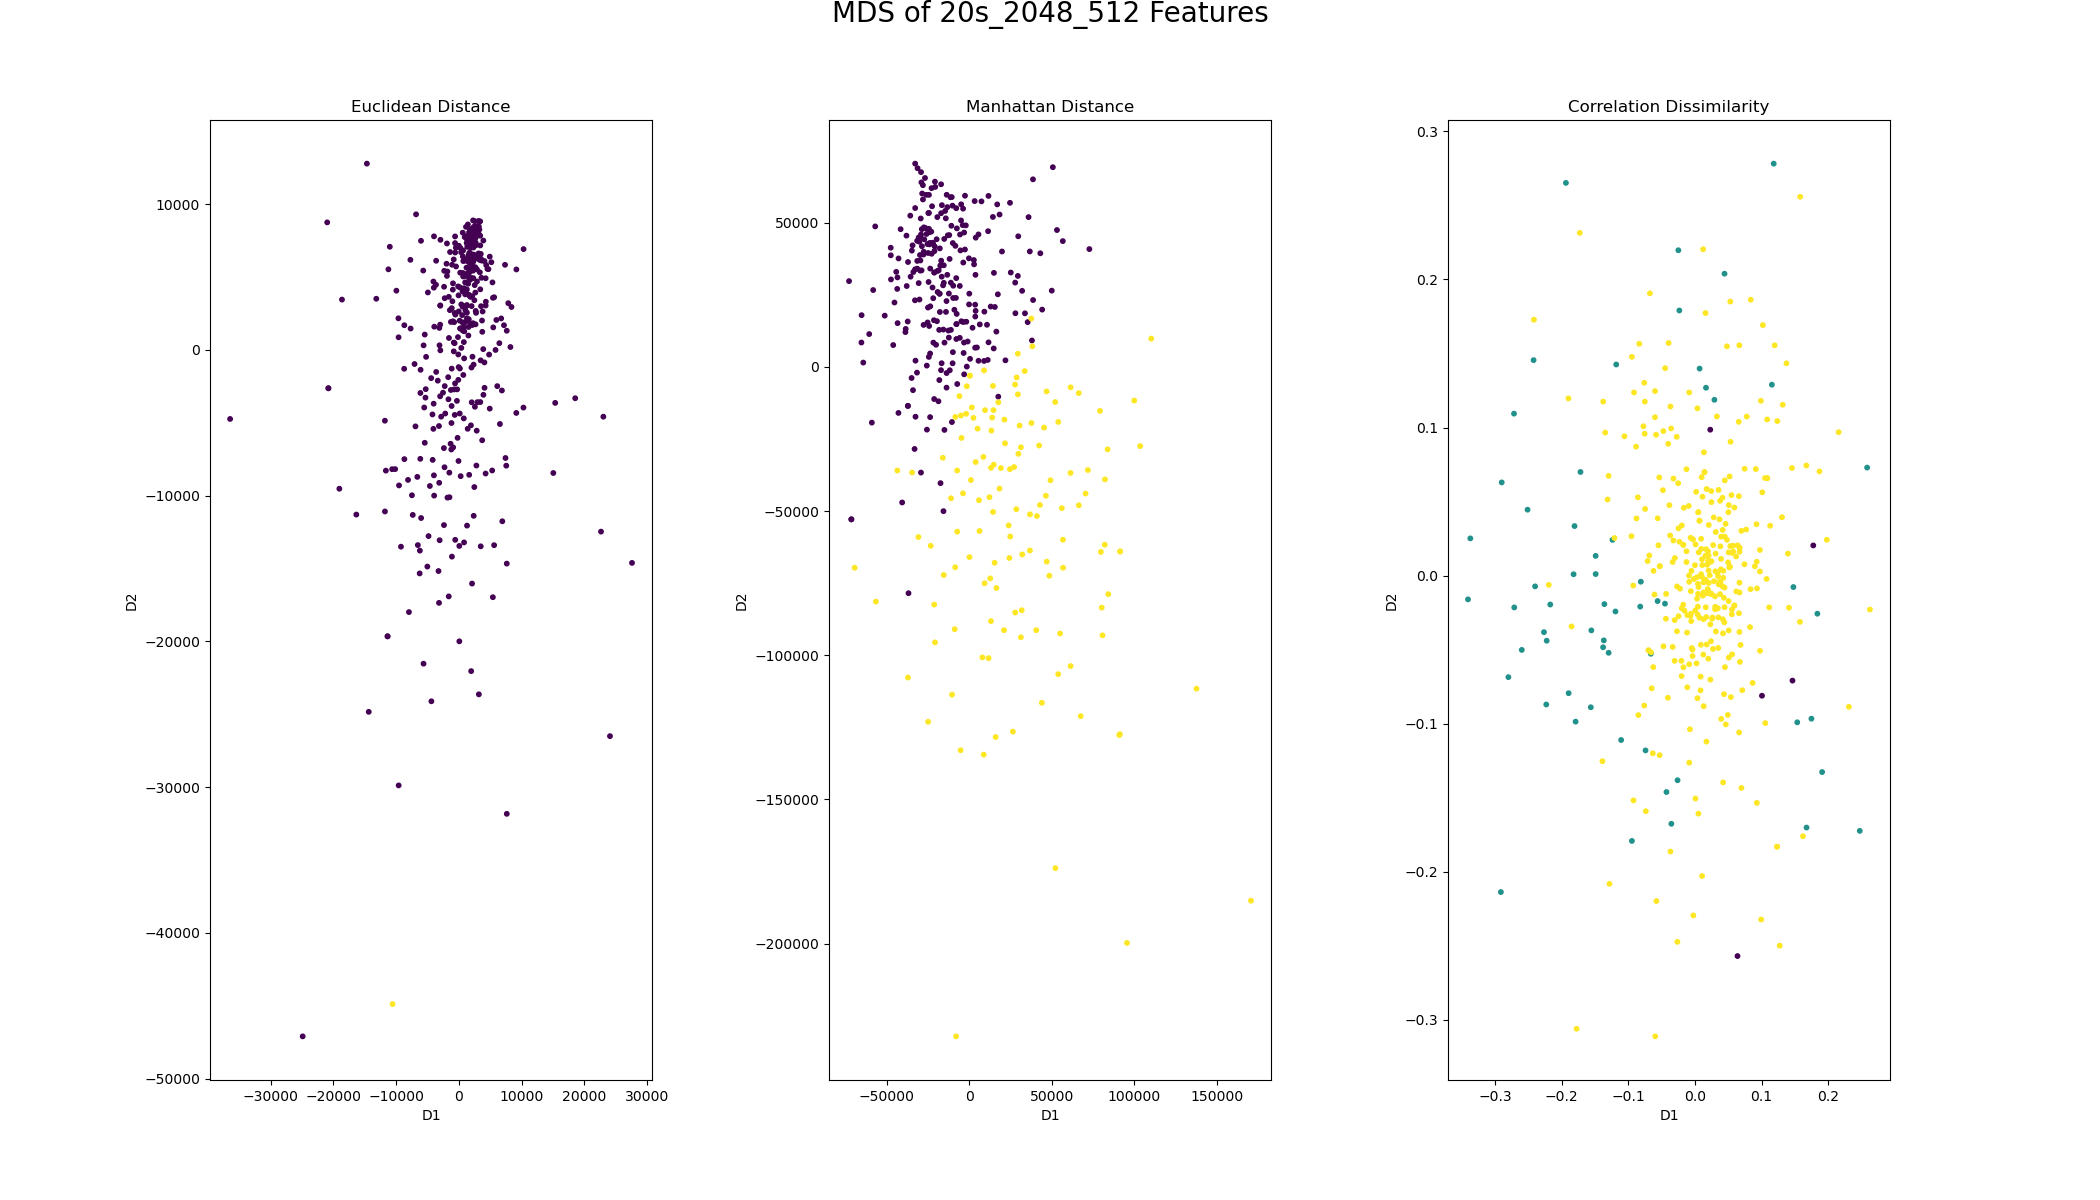
\includegraphics[width=0.9\linewidth]{../Statistical_Sciences_template/figure/MDS of 20s_2048_512 Features Using Complete Linkage.png}
	\caption{The plot is the two-dimensional MDS results of the dataset within 20 seconds, 2048 samples of frame length and 512 samples of hop length for Euclidean distance, Manhattan distance and Correlation dissimilarity respectively.}
	\label{fig:MDS of 20s_1024_256 Features Using Complete Linkage}
\end{figure}
\noindent This figure shows the comparison of clustering results based on different distance metrics (Euclidean distance, Manhattan distance, and correlation dissimilarity) when using the complete linkage method for hierarchical clustering analysis. Through observation, it can be found that the choice of distance function has a decisive impact on the rationality of clustering structure.\\
\\
When using Euclidean distance, clustering algorithms produce very imbalanced partitioning results: data is extremely divided into two clusters, where one cluster (purple points) contains the vast majority of samples, while the other cluster (yellow point) is composed of only one isolated dot. This highly skewed clustering result indicates that Euclidean distance may be overly sensitive to outliers and the high dimensions on this dataset, leading to clustering failure and inability to reflect the true natural structure of the data.\\
\\
In contrast, the performance of Manhattan distance is more robust, and its clustering results form two clusters with clear differences: the purple cluster has dense sample points and high similarity, indicating that they are highly consistent in MFCCs statistical features. The sample points of the yellow cluster are more sparsely distributed and have significant feature differences, which may correspond to music segments where certain acoustic features deviate significantly. Although clustering labels cannot be directly mapped to music genres, this result reveals the distribution pattern of MFCC feature space, providing a reference for music similarity analysis.\\
\\
The third figure shows the clustering results based on correlation dissimilarity, which has a more complex and interpretable structure. The algorithm divides the data into three clusters: the yellow cluster serves as the core group, presenting a typical center dense and edge sparse distribution pattern, implying that most music samples have commonalities in MFCC features. The purple cluster composed of five points on the right has significant consistency in the D1 dimension (all samples have values greater than 0 in this dimension), indicating that these samples may share a specific acoustic feature. The scattered blue-green clusters represent samples with relatively unique features. Although they have some similarities with the main data, their positions in the overall feature space may be relatively isolated.\\
\\
In order to comprehensively evaluate different hierarchical clustering methods, we tested various linkage methods including single linkage, complete linkage, and average linkage on the generated datasets in Section \ref{subsec:FP}. The whole results of these experiments can be found in Appendix \ref{app:C}. The experimental results show that the clustering effect is extremely sensitive to the choice of connection method, and in some cases, catastrophic results  may occur, such as extremely imbalanced cluster distribution or meaningless partitioning that completely violates the true structure of the data. These abnormal phenomena are particularly common in single and average linkage methods, while complete linkage methods, although relatively robust to noise, may produce suboptimal solutions in high-dimensional data.\\
\\
\begin{figure}[h!]
	\centering
	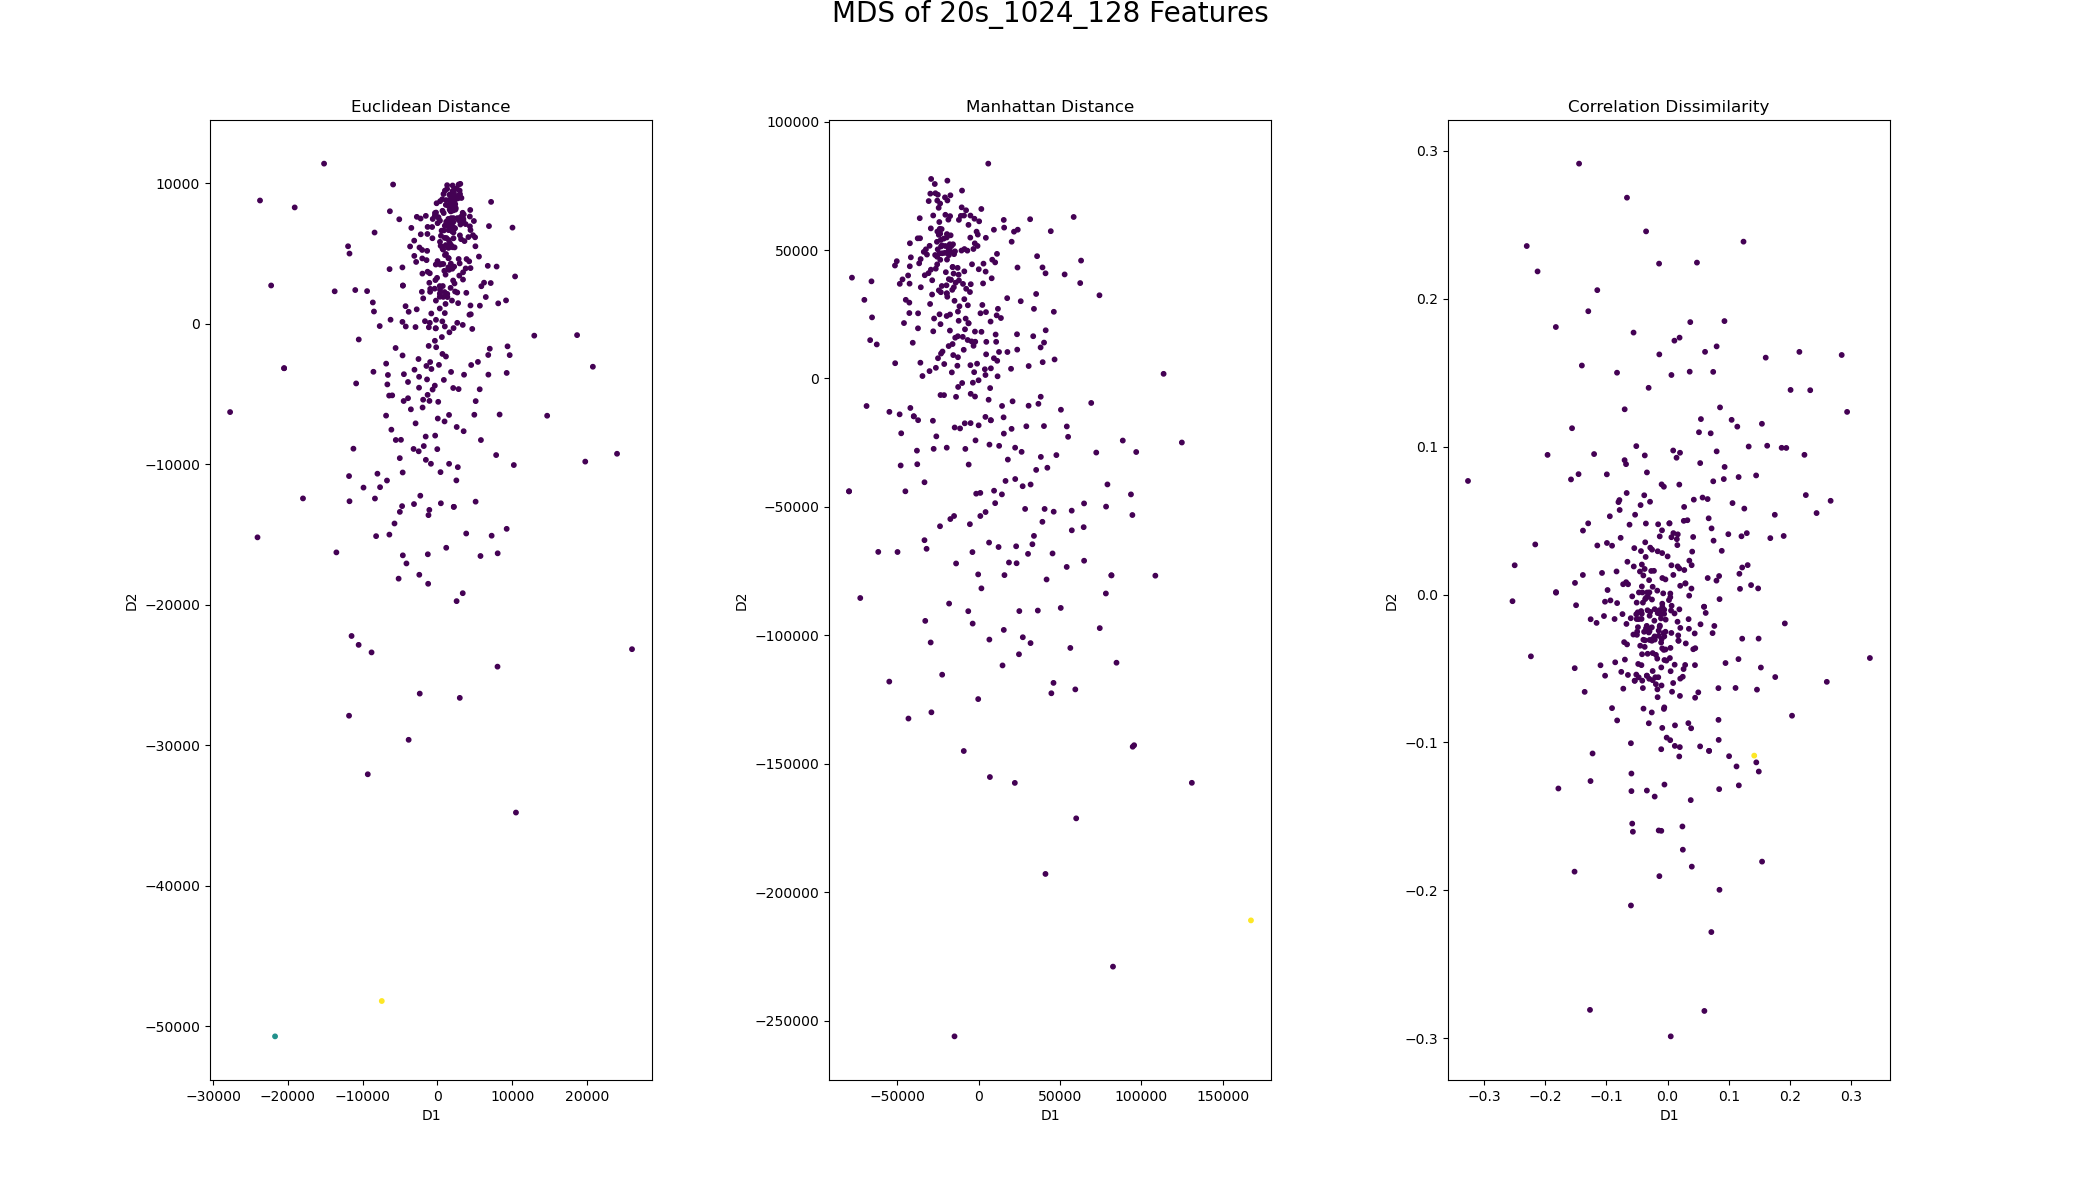
\includegraphics[width=0.9\linewidth]{../Statistical_Sciences_template/figure/MDS of 20s_1024_128 Features Using Single Linkage.png}
	\caption{The plot is the two-dimensional MDS results of the dataset within 20 seconds, 1024 samples of frame length and 128 samples of hop length.}
	\label{fig:MDS of 20s_1024_256 Features Using Single Linkage}
\end{figure}
\noindent The Figure \ref{fig:MDS of 20s_1024_256 Features Using Single Linkage} above is a typical result within single linkage. We can see from the figure that all clustering results are imbalanced: the vast majority of observations form one cluster, while the other cluster is only consisted of one point. This result has no practical significance other than finding that the observation of cluster composed of single points is far away from most observations. This also directly indicates that in high-dimensional spaces, especially in the case of $p>>n$, single linkage is very unstable and unsuitable.\\
\\
\begin{figure}[h!]
	\centering
	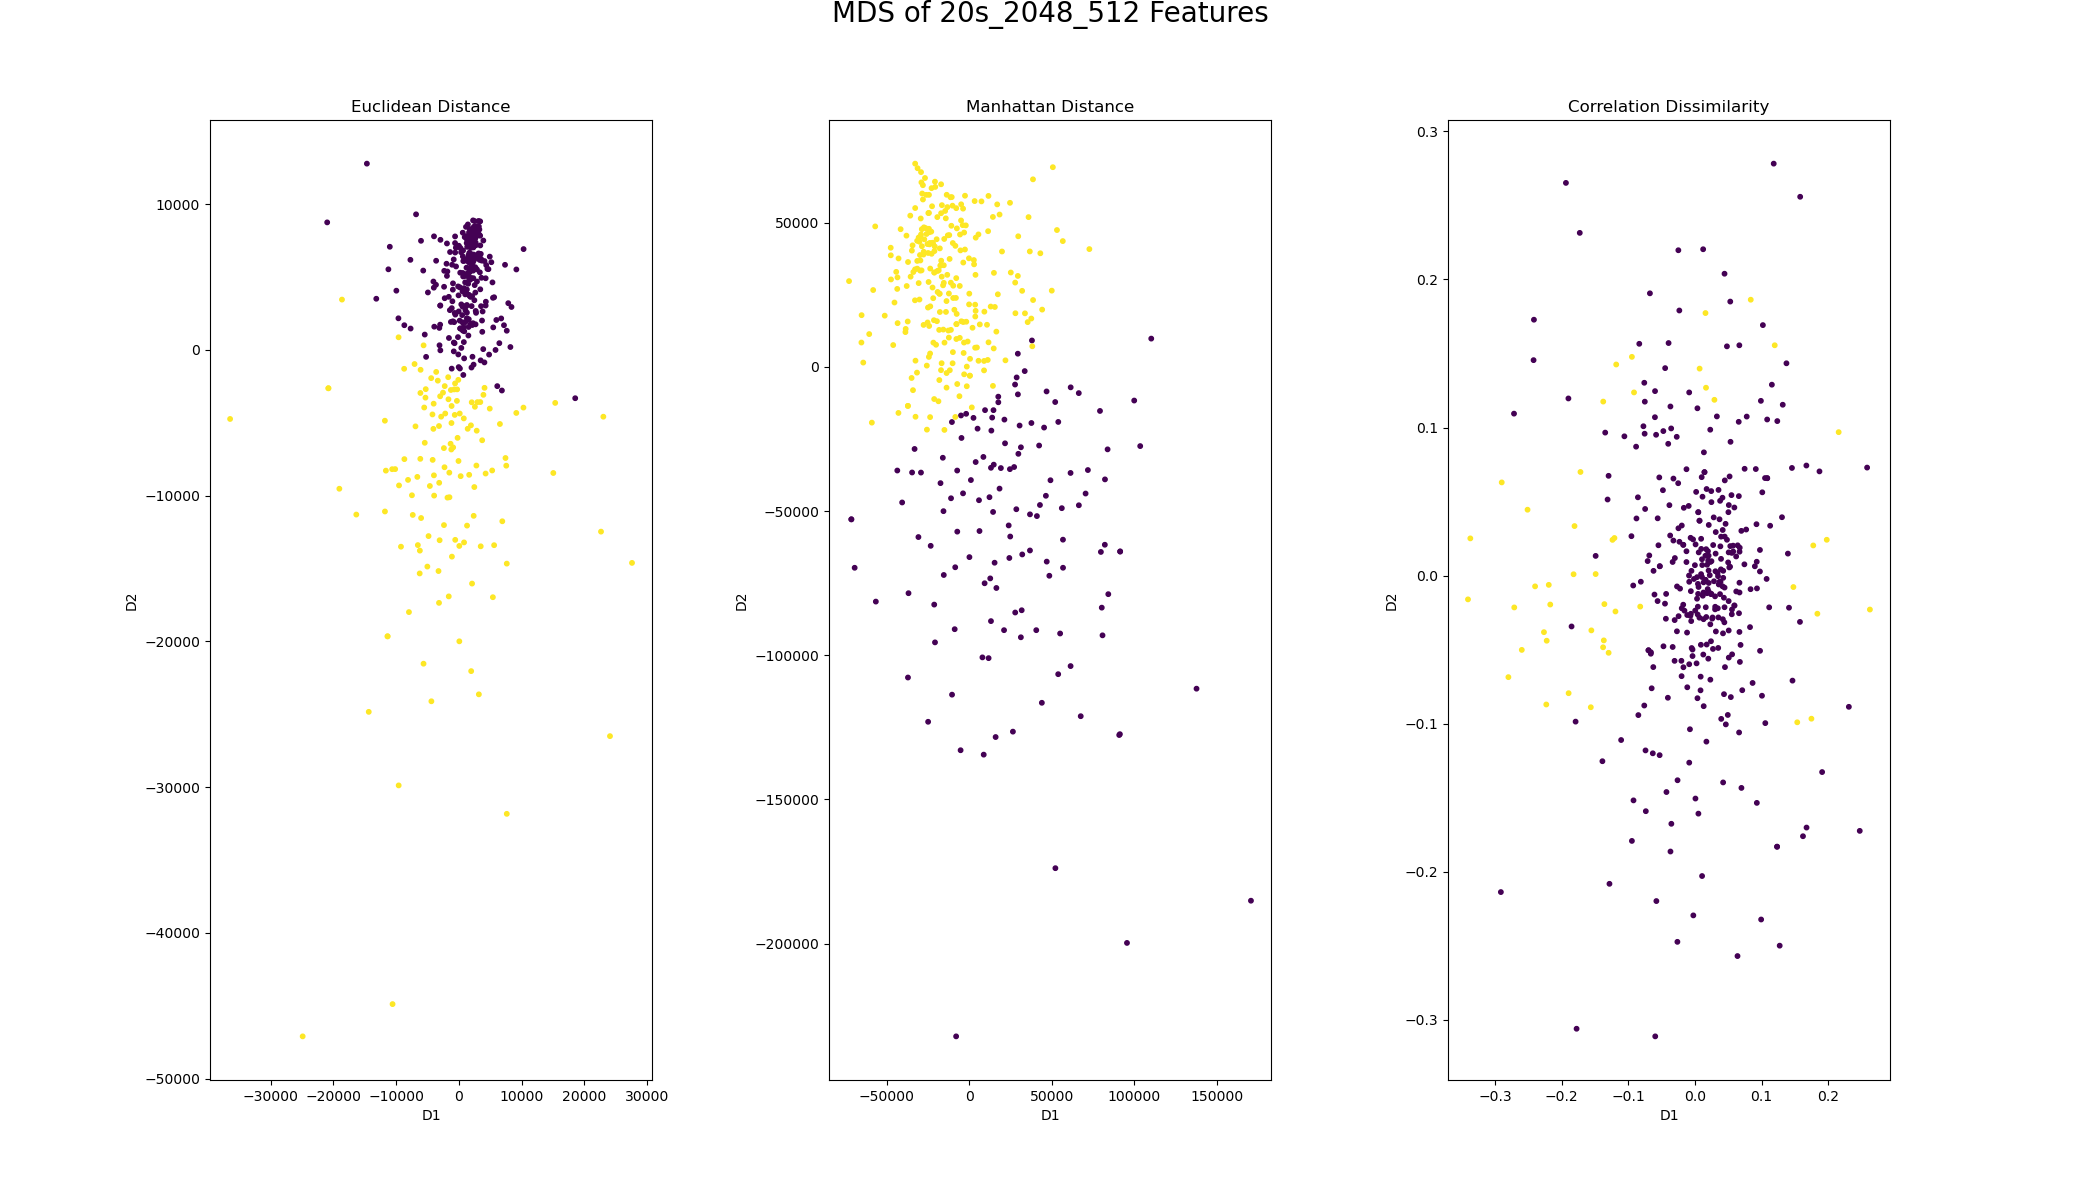
\includegraphics[width=0.9\linewidth]{../Statistical_Sciences_template/figure/MDS of 20s_2048_512 Features Using PAM.png}
	\caption{The plot is the two-dimensional MDS results of the dataset within 20 seconds, 2048 samples of frame length and 512 samples of hop length.}
	\label{fig:MDS of 20s_1024_256 Features Using PAM}
\end{figure}
\noindent The results of PAM clustering are shown in Figure \ref{fig:MDS of 20s_1024_256 Features Using PAM} and are highly consistent with the hierarchical clustering using Manhattan distance combined with complete linkage method. Through the evaluation of ASW, both methods determine that the optimal number of clusters is 2. In the visualization results, the distribution of different clusters is also represented by purple and yellow respectively. The purple cluster shows significant feature homogeneity, and its sample points are closely clustered in the feature space, indicating that these music segments have high similarity in MFCC statistical features. The yellow cluster shows a relatively sparse distribution pattern, suggesting that there is greater variability in the acoustic characteristics of the cluster samples. It is worth noting that although the optimal number of clusters is the same, the boundary of PAM clustering may be clearer than that of hierarchical clustering, which provides a supplementary explanation for subsequent classification tasks such as distance based KNN.\\
\\
\begin{figure}[h!]
	\centering
	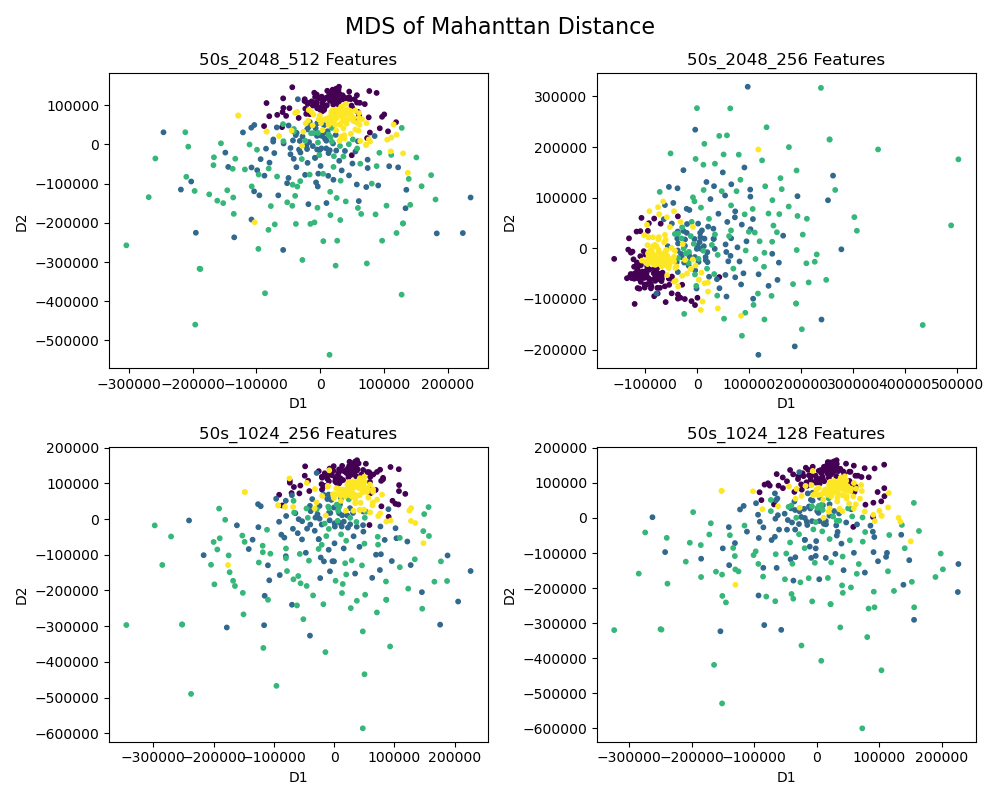
\includegraphics[width=0.9\linewidth]{../Statistical_Sciences_template/figure/MDS of Mahanttan Distance 50s.png}
	\caption{This figure is the MDS visualization of Manhattan distances for the four datasets of 50 seconds}
	\label{fig:MDS of Mahanttan Distance 50s}
\end{figure}
\noindent Unfortunately, these statistical features based on MFCCs cannot clearly reflect the true classification of music genres. From the visualization results in Figure \ref{fig:MDS of Mahanttan Distance 50s} and Figure \ref{fig:MDS of Correlation Dissimilarity 50s}, it can be observed that the acoustic characteristics of different schools show complex distribution patterns in the feature space. In Figure \ref{fig:MDS of Mahanttan Distance 50s}, the purple observation points representing classical music are highly concentrated in the core area with the highest density, while the adjacent yellow observation points (corresponding to disco music) are very close in the feature space, showing amazing similarity. It's worth to note that the blue-green and green observation points representing hiphop and metal music respectively are not only relatively scattered, but also show an obvious crisscross state, which can hardly be effectively distinguished through the boundary. The MDS dimension reduction results in Figure \ref{fig:MDS of Correlation Dissimilarity 50s} also confirm similar findings: although purple observation points (classical music) are distributed at the upper and lower ends of the graph due to the directionality generated by the dimension reduction algorithm (the difference in direction does not change the topology between observations), their overall dispersion is high. The yellow observation point (disco) is still located in the transition area between purple and other observation points. The blue-green and green observations (hiphop and metal) are more mixed.\\
\\
\begin{figure}[h!]
	\centering
	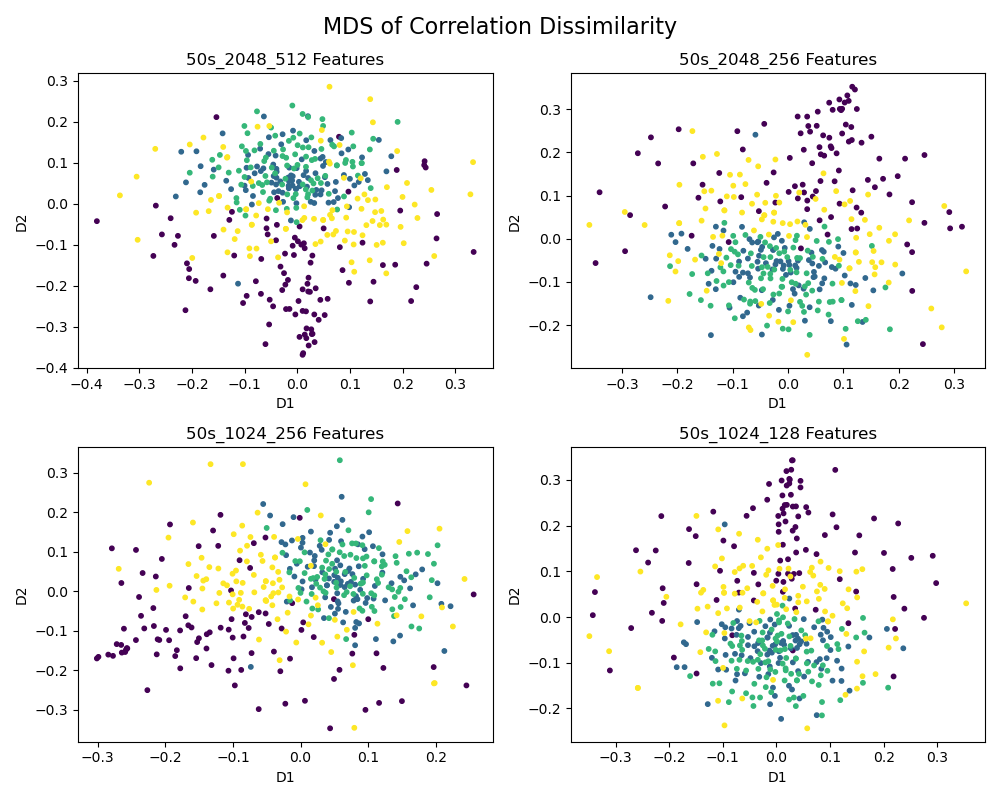
\includegraphics[width=0.9\linewidth]{../Statistical_Sciences_template/figure/MDS of Correlation Dissimilarity 50s.png}
	\caption{This figure is the MDS visualization of correlation dissimilarity for the four datasets of 50 seconds}
	\label{fig:MDS of Correlation Dissimilarity 50s}
\end{figure}
\section{Supervised Statistical Models for Classification}
This section focuses on the complete steps of fitting a supervised learning models based on MFCC statistical features, including model building strategies and specific implementation steps, and evaluates the model performance. In particular, the study focuses on the performance differences between traditional machine learning methods and shapelet tree-based algorithms in music genre classification. In the comparative analysis, we focus on the differences between the two methods in feature representation and classification performance.\\
\\
In terms of the data set partitioning strategy, this study adopts a special processing method that is different from canonical machine learning practices. Considering that the total research data is 400 observations, of which classical, disco, hiphop and mental each accounts for 100. Based on the characteristics of the algorithm and the limitation of computing resources, the data partitioning scheme I designed is as follows: first, 200 samples (accounting for 50\% of the total) are randomly selected from the overall dataset as the training set, then 100 samples (25\%) are randomly selected for the validation set of model parameter tuning, and finally the remaining 100 samples (25\%) are used as the test set to evaluate the final performance of the model.\\
\\
This unconventional data partitioning strategy is mainly due to the inherent limitations of the shapelet tree-based algorithm in terms of computational efficiency. As described in Section \ref{subsec:limit}, the algorithm exhibits a high computational complexity when processing sequence data, and its time complexity reaches $O(\bar{l}^3n^2)$ level, and it needs to evaluate $\sum_{i=1}^n\sum_{j=3}^{l_i-1} j$ candidate shapelets. This computing characteristic leads to two significant problems: first, there will be a serious memory bottleneck during the model fitting process, which is difficult to avoid even in an environment equipped with high-performance computing hardware; second, because the algorithm itself contains a recursive structure, even with GPU acceleration, the model training process is still very slow. Based on these constraints, in order to achieve a feasible model under limited computing resources, I had to control the size of the training set to 50\% of the total data volume. Although this compromise sacrificed some training sample volume, it effectively guaranteed the practicality of the experiment and the research progress.\\
\\

\begin{figure}[h!]
	\centering
	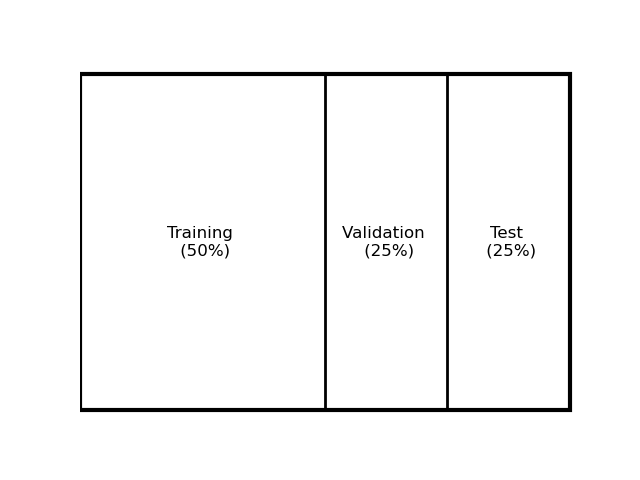
\includegraphics[width=0.9\linewidth]{../Statistical_Sciences_template/figure/Splitting Dataset.png}
	\caption{This is an illustration of how the data set is divided. The training set accounts for 50\% of the total data, the validation set accounts for 25\% of the total data, and the test set also accounts for 25\% of the total data.}
	\label{fig:spliiting}
\end{figure}

\subsection{Fitting the Models}\label{subsec:fitting}
As mentioned in Section \ref{subsec:LR}, Section \ref{subsec:MLR}, Section \ref{subsec:knn} and Section \ref{subsec:SVM} from the previous chapter, this study used methods such as KNN, logistic regression, multinomial logistic regression and support vector machines, and compared the performance of these traditional methods with the results of the shapelet tree-based algorithm. For the traditional statistical learning method, our input is the divided training set mentioned above, and the hyperparameters of various algorithms are tuned through an independent validation set to ensure that each compared model can achieve its optimal performance state, thereby ensuring the reliability of subsequent comparative experiments.\\
\\
Based on the experimental results of Section \ref{subsec:FP}, this study constructed four datasets with different parameters, aiming to explore the key parameter optimization issues in the MFCCs feature extraction process. This strategy enables us to explore the influence of the two key parameters, frame length and hop length, on the model performance. Among them, the choice of frame length directly determines the temporal resolution of time-frequency analysis, while the hop length controls the overlapping part between frames. The optimal combination of these two parameters plays a decisive role in improving the representation ability of speech features. Considering the scale difference problem of the statistical features extracted from MFCC, I adopted a z-score-based normalization method for each variable, which is calculated as 
$$z=\frac{x-\hat{m}}{\hat{s}}$$, 
where $\hat{m}$ represents the sample mean of the feature and $\hat{s}$ represents the sample standard deviation. This normalization process can not only eliminate the dimensional differences between different feature dimensions, but also effectively improve the convergence speed and generalization performance of the model. In order to comprehensively evaluate the influence of data normalization on model performance, I used the standardized MFCCs statistical features for model training on the one hand, and retained the original unstandardized features on the other hand. Thus only the 1-second-long datasets were used for training the model because their dimensions are much lower than that of the 0.4-second-long datasets.\\
\\
When training the KNN classification models, this study examined three different distance metrics, including cosine distance, Manhattan distance, and Euclidean distance. It should be noted that when using cosine distance as a metric, we only used the original statistical feature data that was not standardized for model training, and did not fit a KNN model based on cosine distance for the standardized data. The theoretical basis of this strategy is that z-score standardization, as a linear transformation method, only translates and scales the original data vectors without changing the relative direction relationship of the vectors in the feature space. Since the calculation of cosine distances essentially reflects the cosine values of the angle between vectors, its calculation result is only related to the direction of the vectors, and after L2 norm normalization, the influence of vector length has been completely eliminated. Therefore, standardization does not change the similarity measurement result based on cosine distance, which makes it unnecessary to train a KNN model based on cosine distance after standardization.\\
\\
Based on the above analysis, this experiment adopted the following modeling strategy: for the unstandardized original statistical feature data, we trained a KNN model containing all three distance metrics (cosine distance, Manhattan distance and Euclidean distance); for the standardized data, only the KNN model based on Manhattan distance and Euclidean distance was fitting. Considering that KNN is a typical nonparametric statistical learning method, its model performance mainly depends on the selection of the key hyperparameter $K$, the number of neighbors. Therefore, we adopted a systematic parameter optimization method: in the experiment, we tested integer values of $K$ from 2 to 10, trained the corresponding KNN model for each candidate K value, and evaluated its performance by calculating the classification accuracy of the model on the validation set. Finally, we selected the K value corresponding to the highest classification accuracy on the validation set as the optimal hyperparameter of the model.\\
\\
\\
\\
In the process of training logistic regression and multinomial logistic regression models, this study uniformly adopted L1 penalty for high dimensional data where the number of training set observations $n$ is significantly less than the number of feature variables $p$ (i.e. $n<<p$). This method is chosen because: when the feature dimension $p$ is much larger than the sample size $n$, if the classical maximum likelihood estimation method is directly used for parameter estimation (as described in Section \ref{subsec:LR} and Section \ref{subsec:MLR}), some problems for matrix computation will occur. Specifically, the maximum column rank of the design matrix $X$ is $n$. When $p>n$, the matrix $X^TX$ must be irreversible, resulting in the covariance matrix of the parameter estimation being non positive definite. At this time, there are more than one combinations of regression coefficients that can simultaneously reach the maximum value of the likelihood function or the minimum value of the loss function. From a geometric perspective, the sparsity of data points in high dimensional feature space leads to the existence of multiple hyperplanes that meet the linear separability condition, which directly leads to no unique model solutions. In addition, during the maximum likelihood estimation process, the algorithm can easily pursue the maximization of the likelihood function by making the some regression coefficients corresponding to specific features be infinity, which not only leads to the instability of numerical calculations, but also significantly reduces the parameter convergence speed and even causes divergence.\\
\\
The core advantages of introducing L1 penalty (lasso penalty) are reflected in three aspects: first, by applying L1 penalty, the regression coefficients of some unimportant features are shrunk to zero exactly, thereby achieving feature selection, which is of great value for eliminating redundant features and improving model interpretability; second, the geometric characteristics of L1 penalty (the vertices of the diamond constraint domain are located on the coordinate axis) can effectively compress the size of solution space, and in most cases, many solutions can be converted into a finite number of sparse solutions, and even in some cases, the only optimal solution can be obtained. It should be noted that when there are completely collinear features (such as two completely correlated variables), although L1 penalty cannot completely find the unique solution (it may randomly retain one of the features and discard the other), its solution space dimension has been greatly reduced compared to the original model without any constraints, which still has significant advantages in practical applications. This experiment did not conduct a deep discussion on this extreme case, mainly because the probability of complete collinearity in reality is low.\\
\\
In comparison, although L2 penalty (ridge penalty) can mathematically ensure that parameter estimation has a unique solution, its core disadvantage is that it cannot achieve feature selection——all regression coefficients are proportionally compressed through quadratic penalty terms, resulting in a large number of redundant or noise features still being retained in the model, which not only reduces the interpretability of the model, but may also cause additional variance due to the unimportant noise features. In addition, there are fundamental limitations in the way L2 penalty dealing with collinearity problems: when highly correlated feature groups exist, it tends to retain the regression coefficients of each corresponding variable rather than perform feature selection. More importantly, L2 penalty cannot effectively eliminate the numerical calculation difficulties caused by matrix singularity in high dimensional data, where the model convergence speed may still be seriously affected. Therefore, L2 or elastic net, which includes the L2 penalty term, was not used in this experiment.\\
\\
Another point to note is that in the process of statistical modeling, the selection of regularization parameters has a decisive influence on the performance of the logistic regression model and the multinomial logistic regression model. In other words, the setting of the L1 regularization parameter $\lambda$ is particularly critical. This parameter directly controls how many coefficients of the model will shrink to 0 exactly. The larger the lambda value, the stronger the penalty imposed on the model coefficients, which will cause more coefficients to shrink to 0, thereby effectively reducing the complexity of the model and preventing the occurrence of overfitting. Conversely, when the lambda value is small, the regularization effect is weakened and the model retains more feature information. In particular, when $\lambda=0$, the model will degenerate into a standard logistic regression or multinomial logistic regression form, and no regularization constraints are imposed at this time. In this study, the optimal lambda value was determined using a statistical method based on the performance of the validation set, that is, the classification accuracy of the model on the validation set under different lambda values was evaluated, and the lambda value that maximized the accuracy of the validation set was finally selected as the optimal parameter. It should be noted that since this study uses Python's scikit-learn library to implement model training, the regularization strength is controlled by the parameter $C$ in the LogisticRegression class. From a mathematical perspective, $C$ is the reciprocal of $\lambda$, that is $C=\frac{1}{\lambda}$. This parameterization means that a larger $C$ value corresponds to a smaller regularization strength, while a smaller C value corresponds to a stronger regularization effect.\\
\\
\\
\\
The last traditional statistical learning method used in this study is the Support Vector Machine (SVM), specifically the Linear Support Vector Classifier. In the process of model selection, I experimented with the applicability of various kernel functions, including nonlinear kernel functions such as the Polynomial Kernel and the Gaussian Kernel. However, due to the typical high dimensional features of the data in this study (i.e., the feature dimension p is much larger than the sample size n), the nonlinear kernel function showed a significant overfitting tendency during the training process, and its classification performance was significantly inferior to that of the linear kernel function. Based on the quantitative comparison of the validation results, I finally decided to use only the linear kernel function for subsequent analysis.\\
\\
Considering that each feature variable in the high dimensional data has different scales and distribution ranges, directly using the original data for modeling may cause the optimization algorithm to fail to converge, and also make the model have an unreasonable preference for features with larger dimensions. For this reason, I tried to use the standardized data for model training and subsequent analysis and comparison instead of using the original data. Similar to the logistic regression and multinomial logistic regression models used in this study, the linear support vector classifier also introduces the L1 penalty to reduce the risk of overfitting and enhance the robustness of the model.\\
\\
In terms of the technical details of the model implementation, it should be noted that the linear support vector classifier used in this study is implemented based on the LinearSVC class of the scikit-learn machine learning library in the Python. The algorithm implementation of this class is derived from the LIBLINEAR efficient optimization library developed by Fan et al. (2008). In this article, the loss of the support vector machine is defined as follows:
$$
\min_{\mathbf{w}}\frac{1}{2} \mathbf{w}^T\mathbf{w}+C\sum\xi(\mathbf{w},\mathbf{x},y),
$$
which is corresponding to Equation \eqref{svmL2}. The term "L1-SVM" proposed by Fan et al. in their original paper specifically refers to the support vector machine model using the standard hinge loss function (i.e., L1 loss), that is
$$
\max(1-y\mathbf{w}^T\mathbf{x},0),
$$
which is essentially different from the model used in this study. Although the model actually used in this study also applies the L1 regularization penalty term, its loss function adopts the form of squared hinge (L2 loss), that is
$$
\max(1-y\mathbf{w}^T\mathbf{x},0)^2
$$
In summary, there are two major differences between L1-SVM and the model in this study: one is the penalty term, which is the L2 norm in L1-SVM and the L1 norm in this model; the other is the part of loss function, which is the hinge loss in L1-SVM and the squared hinge loss in this model. Accordingly, the corresponding loss for the model in my study is Equation \eqref{svmL1}, while the loss for L1-SVM corresponds to \eqref{svmL2}.\\
\\
\\
\\
The implementation of the shapelet algorithm in this study uses a completely different technical route from the traditional statistical model method. In the early exploration stage, I first tried to reduce the dimensionality of the original audio signal. Specifically, I used an operation method similar to pooling, that is, to segment the audio signal, extract audio segments of fixed length (including 1 second and 0.4 second duration settings), and then calculate two statistical features of each segment: maximum value (max pooling) and mean (mean pooling). This statistical feature based sequence compression method aims to convert the high-dimensional original audio signal into a low dimensional time series representation, thereby meeting the shapelet algorithm's requirements for the input data dimension.\\
\\
However, after multiple experimental verifications, this strategy showed serious problems in multiple key indicators. During the model training process, when a deeper decision tree structure was used, the model performed well on the training set, with an accuracy generally above 0.7, but the performance on the validation set and test set dropped sharply, with the accuracy mostly less than 0.3, and some models even as low as around 0.2. This huge performance gap indicates that the model has a serious overfitting problem. To improve this situation, I tried to reduce the model complexity (that is, reduce the depth of the tree) by adjusting the model parameters, and also tried to increase the sample size of the training set. Although these adjustments did alleviate the overfitting phenomenon, they led to new problems-the model began to show obvious underfitting characteristics, and the accuracy on the training set, validation set, and test set remained at a low level.\\
\\
This dilemma could not be effectively resolved after many attempts at parameter tuning. Specifically, when trying to find an intermediate parameter setting, the model either still has a certain degree of overfitting or tends to underfit. I realized that this dimensionality reduction strategy based on pooling operations is inherently in conflict with the characteristics of the shapelet algorithm. The shapelet algorithm needs to identify key local subsequence features in the time series, and the shapelets found after the pooling operation are not representative enough. This information loss makes it difficult for the algorithm to find truly discriminative shapelets, which ultimately leads to the complete abandonment of the strategy.\\
\\
Another important idea proposed in this study comes from the observation and analysis of MFCCs features. Through the change patterns of MFCCs coefficients shown in Figure \ref{fig:Low MFCCs} and Figure \ref{fig:High MFCCs}, we found that low-frequency cepstral coefficients (especially the first MFCCs) showed significant differences in the time dimension, while high-frequency cepstral coefficients showed a highly consistent change trend. This obvious difference in spectral characteristics prompted us to form a key hypothesis: low-frequency cepstral coefficients are likely to contain the most representative shapelet patterns due to their more significant temporal variation characteristics and stronger discrimination. Based on this important discovery, I decided to use the mean sequence of the first MFCCs as the basic data for model training. The specific implementation method is as follows: in the feature engineering processing stage, I calculated the mean of 50 first MFCCs for each 0.4 second analysis window, and these processed mean sequences constituted the core input data for subsequent shapelet model training. That is to say, in the results of feature project in Section \ref{subsec:FP}, the mean of the MFCCs data of the corresponding 0.4 second analysis window is used to train the model. Because the audio data is sampled from the 5th second for 20 seconds, each observation has a length of 20 seconds, so this feature project will generate a feature time series of length 50, and the training of the shapelet tree-based algorithm model is based on these sequences of length 50. This modeling strategy based on specific frequency band features not only retains the most discriminative temporal feature information, but also achieves reasonable data dimensionality reduction through mean processing.\\
\\
\subsection{Results and Performance}\label{subsec:performance}
After all models were trained with the training set and the validation set parameters were optimized, the results are shown in the following table. In the table, std represents the standardized data, the first number represents the frame length, and the second number represents the hop length.\\
\\
Table \ref{table:KNN} shows in detail the classification performance of the dataset after feature project and its standardized version on the test set after training using KNN algorithm. First, as mentioned in the beginning of Section \ref{subsec:fitting}, the calculation results of cosine distance are not affected by data standardization due to its inherent scale invariance, so the results of the standardized dataset are not shown Table \ref{table:KNN}.\\
\begin{table}[H]
	\centering
	\caption{Performances of KNN Algorithm}
	\begin{tabularx}{\linewidth}{>{\raggedright\arraybackslash}X *{3}{>{\centering\arraybackslash}m{3.5cm}}}
		\toprule
		Data Set     & KNN with Cosine & KNN with Euclidean & KNN with Manhattan  \\ \midrule
		2048 512     & 0.48            & 0.61               & 0.75                              \\
		2048 256     & 0.52            & 0.65               & 0.72                              \\	
		1024 256     & 0.50            & 0.57               & 0.76                              \\	
		1024 128     & \textbf{0.43}   & 0.56               & 0.77                              \\
		std 2048 512 &             & 0.77                   & 0.8                              \\
		std 2048 256 &             & 0.8                    & 0.8                              \\	
		std 1024 256 &             & 0.82                   & 0.87                              \\	
		std 1024 128 &             & 0.8                    & 0.83                              \\ \bottomrule
	\end{tabularx}
	\label{table:KNN}
\end{table}

\noindent In terms of specific performance, the experimental results of the KNN model show significant differences. When the dataset with 1024 samples of frame length and 128 hop length is applied within the cosine distance metric, the model performs the worst, with a test set accuracy of only 0.43, which is significantly lower than the model performance under other configuration conditions. In sharp contrast, when the standardized dataset with 1024 samples of frame length and 256 hop length is applied the Manhattan distance metric, the model performs the best of all KNN models, with a test set accuracy of 0.87, which is nearly double the worst configuration.\\
\\
By comparing and analyzing the datasets with different parameter configurations, the following important findings can be drawn: first, the parameter differences of frame length and hop length have relatively limited influence on the performance of the KNN model, in other words, the performance of the models under different parameter configurations of feature project is not much different. For example, the test set accuracy of the standardized data set in the KNN model based on Manhattan distance is more than 0.8, and the test set accuracy of the unstandardized data set in the KNN model based on Euclidean distance is also around 0.61. The differences between them are not obvious. However, it is worth noting that data standardization has a significant effect on improving model performance. Specifically, whether Euclidean distance or Manhattan distance is used as the distance metric, the standardized data set can bring significant accuracy improvement, and this phenomenon has been verified in all the datasets. Further analysis of the performance differences of different distance metrics can reveal a stable and significant rule: under the condition of fixed frame length and hop length, the performance of the distance metric shows obvious gradient differences, with Manhattan distance performing the best, Euclidean distance second, and cosine distance performing the worst. In addition, experimental results also show that the choice of distance metric influence model performance even more than the choice of feature project parameters.\\
\\
Table \ref{table:L1penalty} shows the performance comparison of three classical classification models using L1 penalty constraints, including logistic regression, multinomial logistic regression, and SVM (linear support vector classifier), on the unstandardized dataset and the standardized dataset. It should be noted that due to the serious convergence problem when training the linear support vector classifier on the unstandardized dataset (no matter how many iterations were taken), the test results under this condition are not reliable, so they are not presented in the table. In addition, although the traditional logistic regression is mainly applicable to binary classification scenarios, this study uses the "one-vs-rest" strategy to construct a combination of four independent logistic regression models, thereby achieving multi-classification capabilities. This strategy can be easily achieved by the scikit-learn class LogisticRegression() within the solver "liblinear" in Python, which is also a part of the work by Fan et al. (2008).\\

\begin{table}[H]
	\centering
	\caption{Performances of Algorithms with L1 Penalty}
    \begin{tabularx}{\linewidth}{>{\raggedright\arraybackslash}X *{3}{>{\centering\arraybackslash}m{3.5cm}}}
	\toprule
Data Set     &  LR & Multinomial LR & Linear SVM  \\ \midrule
2048 512     & 0.74       & 0.65            &                                            \\
2048 256     & 0.77       & 0.65            &                                            \\	
1024 256     & 0.78       & 0.6            &                                            \\	
1024 128     & 0.73       & 0.65            &                                            \\
std 2048 512 & 0.72       & 0.82            & 0.83                                            \\
std 2048 256 & 0.67       & 0.86            & 0.82                                           \\	
std 1024 256 & 0.67       & \textbf{0.89}             & 0.81                                           \\	
std 1024 128 & 0.67        & \textbf{0.89}           & 0.86                                           \\ \bottomrule
	\end{tabularx}
	\label{table:L1penalty}
\end{table}

\noindent Several important findings can be drawn from the experimental results. First, the impact of data standardization on model performance shows obvious differences. The standardized data set showed excellent classification performance on both the multinomial logistic regression and SVM models, and the test set accuracy exceeded 0.8. It is particularly noteworthy that the standardized data set with 1024 frame length and 128 jump length combined with the multinomial logistic regression model achieved the best classification effect, with a test accuracy of 0.89. Analyzing the impact of standardization on different models, we found an interesting phenomenon: standardization caused the performance of the logistic regression combination model to decline (an average decrease of about 0.07), but significantly improved the accuracy of the multinomial logistic regression model (an average increase of about 0.2).\\
\\
In the performance comparison of different models, we observed the following pattern: for the standardized data set, the performance of the logistic regression combination is better than that of the multinomial logistic regression, with the test accuracy of the former being stable at above 0.73, while the latter is concentrated at 0.65. However, on the standardized data set, this superiority-inferiority relationship is reversed: the accuracy of the multinomial logistic regression is over 0.82, significantly higher than the highest accuracy of 0.72 of the logistic regression combination. The standardization process effectively eliminates the performance bottleneck of the multinomial logistic regression. It is worth noting that under standardized conditions, the performance of the multinomial logistic regression and the linear support vector classifier is quite close, with the accuracy difference between the two not exceeding 0.04, and the performance of the two on the test set is alternately leading. Based on the experimental results above, we can draw the following conclusions: under the conditions of standardized data, the performance of the three models presents a hierarchical structure. Logistic regression performs the worst, while multinomial logistic regression and SVM models show similar and significantly superior performance.\\
\\
Table \ref{table:best} shows the evaluation results of the best model, i.e. the multinomial logistic regression trained on the standardized dataset with 1024 frame length and 128 hop length, on the test set, covering all four categories (classical, disco, hiphop, and mental), as well as the overall macro-average and weighted average evaluation scores. From the results, the model performs best on classical, with precision, recall, and F1-score all reaching 1.00, indicating that the model can correctly identify all samples in this category without misclassification or omission. The performance of hiphop is also relatively stable, with all three indicators being 0.89, indicating that the model has a relatively balanced classification effect on it. In contrast, there are some fluctuations in the indicators of disco and mental: the precision of disco is high (0.95), but the recall rate is a little bit lower (0.72), which means that nearly 28\% of the samples of this category are missed by the model, and the shortcoming of the recall lowers the F1-score. While mental is the opposite, with a recall rate of 0.95, indicating that the model has a strong coverage of this category, but the precision rate is only 0.75, which may misclassify other categories as this category, resulting in more false positives. Overall, the macro average and weighted average F1-scores of the model are both 0.89, which is the harmonic average of precision and recall, indicating that the overall performance is relatively stable and there is no obvious deviation due to the difference in the number of samples (the support number of each category is between 22 and 27).\\

\begin{table}[H]
	\centering
	\caption{Performance of Multinomial LR within Standard 1024 128 Dataset}
	\begin{tabularx}{\linewidth}{>{\raggedright\arraybackslash}X *{4}{>{\centering\arraybackslash}m{2.8cm}}}
		\toprule
		&  Precision & Recall & F1-score & Support \\ \midrule
		Classical     &  1.00  & 1.00  & 1.00  &  26    \\
		Disco     &  0.95  & 0.72  & 0.82  &  25  \\
		Hiphop     &  0.89  & 0.89  & 0.89  &  27   \\
		Mental     &  0.75  & 0.95  & 0.84  &  22   \\
		\\
		macro avg  & 0.90 & 0.89 &0.89 & 100 \\
		weighted avg  & 0.90 & 0.89 &0.89 & 100 \\  \bottomrule
	\end{tabularx}
	\label{table:best}
\end{table}

\noindent Table \ref{table:shapeletmodels} shows the classification accuracy of the shapelet tree-based algorithm on the test set. Compared with the traditional statistical learning methods such as multinomial logistic regression and SVM models mentioned above, the classification performance of this algorithm is relatively weak. The best model trained on the dataset within 2048 frame length and 256 hop length only achieved an accuracy of 0.63. Although this value is significantly lower than the classification results of some other models, the result is significantly different from the null model (random guessing) and is a little better than that of the KNN models using cosine distance, indicating that the algorithm does have a certain degree of discrimination ability. A detailed analysis and discussion of the performance limitations of this algorithm will be carried out in Section \ref{subsec:explaination}, including a comparative study with other algorithms and a discussion of potential improvement directions.\\


\begin{table}[H]
	\centering
	\caption{Performances of Shapelet Tree-based Algorithm}
	\begin{tabularx}{\linewidth}{>{\raggedright\arraybackslash}X *{4}{>{\centering\arraybackslash}m{3cm}}}
		\toprule
		Data Set     &  2048 512 & 2048 256 & 1024 256 & 1024 128 \\ \midrule
		Accuracy     & 0.55      & 0.63     & 0.51     & 0.53    \\ \bottomrule
	\end{tabularx}
	\label{table:shapeletmodels}
\end{table}

\noindent Table \ref{table:bestshapelet} shows the multi-classification performance evaluation results of the shapelet tree-based algorithm on the dataset within 2048 frame length and 256 hop length. From the comprehensive performance of precision, recall, and F1-Score, the performance of the model in different categories varies significantly, and the overall performance is moderate. The macro average and weighted average are both 0.63 to 0.64, indicating that the model's capabilities need to be improved.\\
\\
Classical performs best, with a precision of 1.00, which means that all samples predicted by the model as classical do belong to this category without misclassification. However, its recall rate is 0.85, indicating that 15\% of classical samples are still misclassified into other categories, probably because the features of these samples partially overlap with other music types. Despite this, classical's F1-score is 0.92, the highest among the four categories, reflecting the high reliability of its prediction results. In contrast, disco performed the worst, with a precision of only 0.47, indicating that the model had a high misclassification rate when predicting disco, and more than half of the predictions may be wrong. At the same time, its recall rate was as low as 0.32, which means that 68\% of Disco samples were not correctly identified. This combination of low precision and low recall resulted in an F1-score of only 0.38 for disco, indicating that the model had serious difficulties in identifying this category.\\

\begin{table}[H]
	\centering
	\caption{Performances of Shapelet within 2048 256 Dataset}
	\begin{tabularx}{\linewidth}{>{\raggedright\arraybackslash}X *{4}{>{\centering\arraybackslash}m{2.8cm}}}
		\toprule
		&  Precision & Recall & F1-Score & Support \\ \midrule
		Classical     &  1.00  & 0.85  & 0.92  &  26    \\
		Disco     &  0.47  & 0.32  & 0.38  &  25  \\
		Hiphop     &  0.52  & 0.63  & 0.57  &  27   \\
		Mental     &  0.57  & 0.73  & 0.64  &  22   \\
		\\
		macro avg  & 0.64 & 0.64 &0.63 & 100 \\
		weighted avg  & 0.64 & 0.64 &0.63 & 100 \\ \bottomrule
	\end{tabularx}
	\label{table:bestshapelet}
\end{table}

\noindent The performance of the hiphop and mental categories was at an intermediate level. Hiphop had a precision of 0.52, a recall of 0.63, and an F1 score of 0.57, indicating that the model had average recognition ability for it, with some misclassification and misidentification. It is worth noting that the recall rate of hiphop is higher than the precision rate, indicating that the model tends to classify more samples as hiphop, but nearly half of them may be wrong. The recall rate of the mental is high (0.73), but the precision rate is only 0.57, which means that although the model can capture most of the mental samples, it is also easy to misclassify the samples from other categories as mental, resulting in more false positives. This imbalance makes its F1 score 0.64, which is better than hiphop and disco, but still not ideal.\\
\\
Overall, the macro average and weighted average are both around 0.64, and the support shows that the sample size of each category is relatively balanced (between 22 and 27), indicating that the performance difference of the model is not caused by data imbalance, but is more likely related to the limitations of feature extraction or the algorithm itself. In particular, the significant shortcomings of the disco category drag down the overall performance. Overall, the current model performs well on classical, but there is still much room for improvement in other categories.\\
\\

\subsection{Explainations of the Models}\label{subsec:explaination}
We can see from Table \ref{table:KNN} that among all the KNN model evaluations, the model using Manhattan distance as the metric exhibits the best classification performance on the standard dataset with 1024 frame length and 256 hop length, with a test set accuracy of 0.87, which is higher than the performance of other KNN models. And as described in Section \ref{subsec:performance}, when the model uses L1 distance, regardless of whether the data is standardized, its results on the test set are better than those using Euclidean distance, and this advantage remains consistent under different parameter configurations.\\
\\
This may be because the Manhattan distance is more robust in feature space, especially in high-dimensional space, while the Euclidean distance or other Minkowski distances with p>2 are not as robust as the Manhattan distance because they use exponentiation operations, which easily amplifies the impact of individual extreme observations. As a result, individual observations in high-dimensional space greatly affect the structure of the model.\\
\\
Moreover, when $p>>n$, the sample points are sparse in the feature space, which may cause the Euclidean distance to not be a good measure of the difference between points. Just like the results of clustering using the Euclidean distance in Section \ref{subsec:clustering}, almost all the results are two clusters: one is composed of the vast majority of observations, and the other is only one observation, such as the result of Euclidean clustering in Figure \ref{fig:MDS of 20s_1024_256 Features Using Complete Linkage}. The clustering results can further illustrate from the side that the Euclidean distance has a poor distinction between samples in high-dimensional space. The Euclidean distance between sample points will approach almost the same value, which is difficult to reflect the differences between samples. As a result, similar phenomena lead to poor results of the KNN model under the Euclidean distance. On the contrary, the Manhattan distance has some obvious distinction between samples in the clustering model, and the clustering results are meaningful, such as the Manhattan clustering results in Figure \ref{fig:MDS of 20s_1024_256 Features Using Complete Linkage}. This more discriminating result makes the KNN model using the Manhattan distance perform better than that using the Euclidean distance.\\
\\
Figure \ref{fig:MLRstdcoef} is the heatmap of coefficients of the multinomial logistic regression models trained on the standardized dataset. In this visualization, the white area indicates that the regression coefficient at the corresponding variable is zero, while the color depth is positively correlated with the absolute value of the coefficients. From this heatmap, we can observe that the L1 penalty term does effectively achieve the sparse features of the model coefficients, and the regression coefficients of most variables are compressed to zero exactly. This feature significantly reduces the adverse influence of high dimensional data on model complexity. It is also worth noting that among all the multinomial logistic regression models fitted on standardized data, the model based on the dataset with frame length 2048 and hop length 512 performs relatively poor. From the intuitive presentation of Figure \ref{fig:MLRstdcoef}, we can see that the coefficients' matrix of this dataset presents the most sparse distribution features, while the coefficient distribution of the other three models is more dense. By calculation, we can find that among the four regression models, the proportion of non-zero coefficients of the dataset with frame length 2048 and hop length 512 is about 0.040, while the proportion of non-zero coefficients in the remaining three datasets is about 0.268, which is much higher than that of the first one. This phenomenon provides a reasonable explanation for the difference in model performance: in the dataset with frame length 2048 and hop length 512, due to the great effect of the L1 penalty term, a large number of coefficients are forced to shrink exactly to zero, and these eliminated coefficients actually contain some feature information with predictive value. In other words, the model may have excessively excluded some variables with discriminative ability during the feature selection process, causing a slight underfitting problem. In contrast, the other three models retain more non-zero coefficients and can make more full use of the effective information in the data, thus obtaining relatively better prediction performance. This difference further verifies the trade-off between regularization and model complexity: although a L1 penalty can effectively control model complexity, it may lead to the loss of valuable information; while moderately relaxing the regularization constraint helps to improve the expressive power of the model. In addition, this phenomenon also suggests that the MFCCs of the dataset with frame length 2048 and hop length 512 may have slightly different feature distribution features from other datasets, making it more sensitive to L1 penalty. \\

\begin{figure}[H]
	\centering
	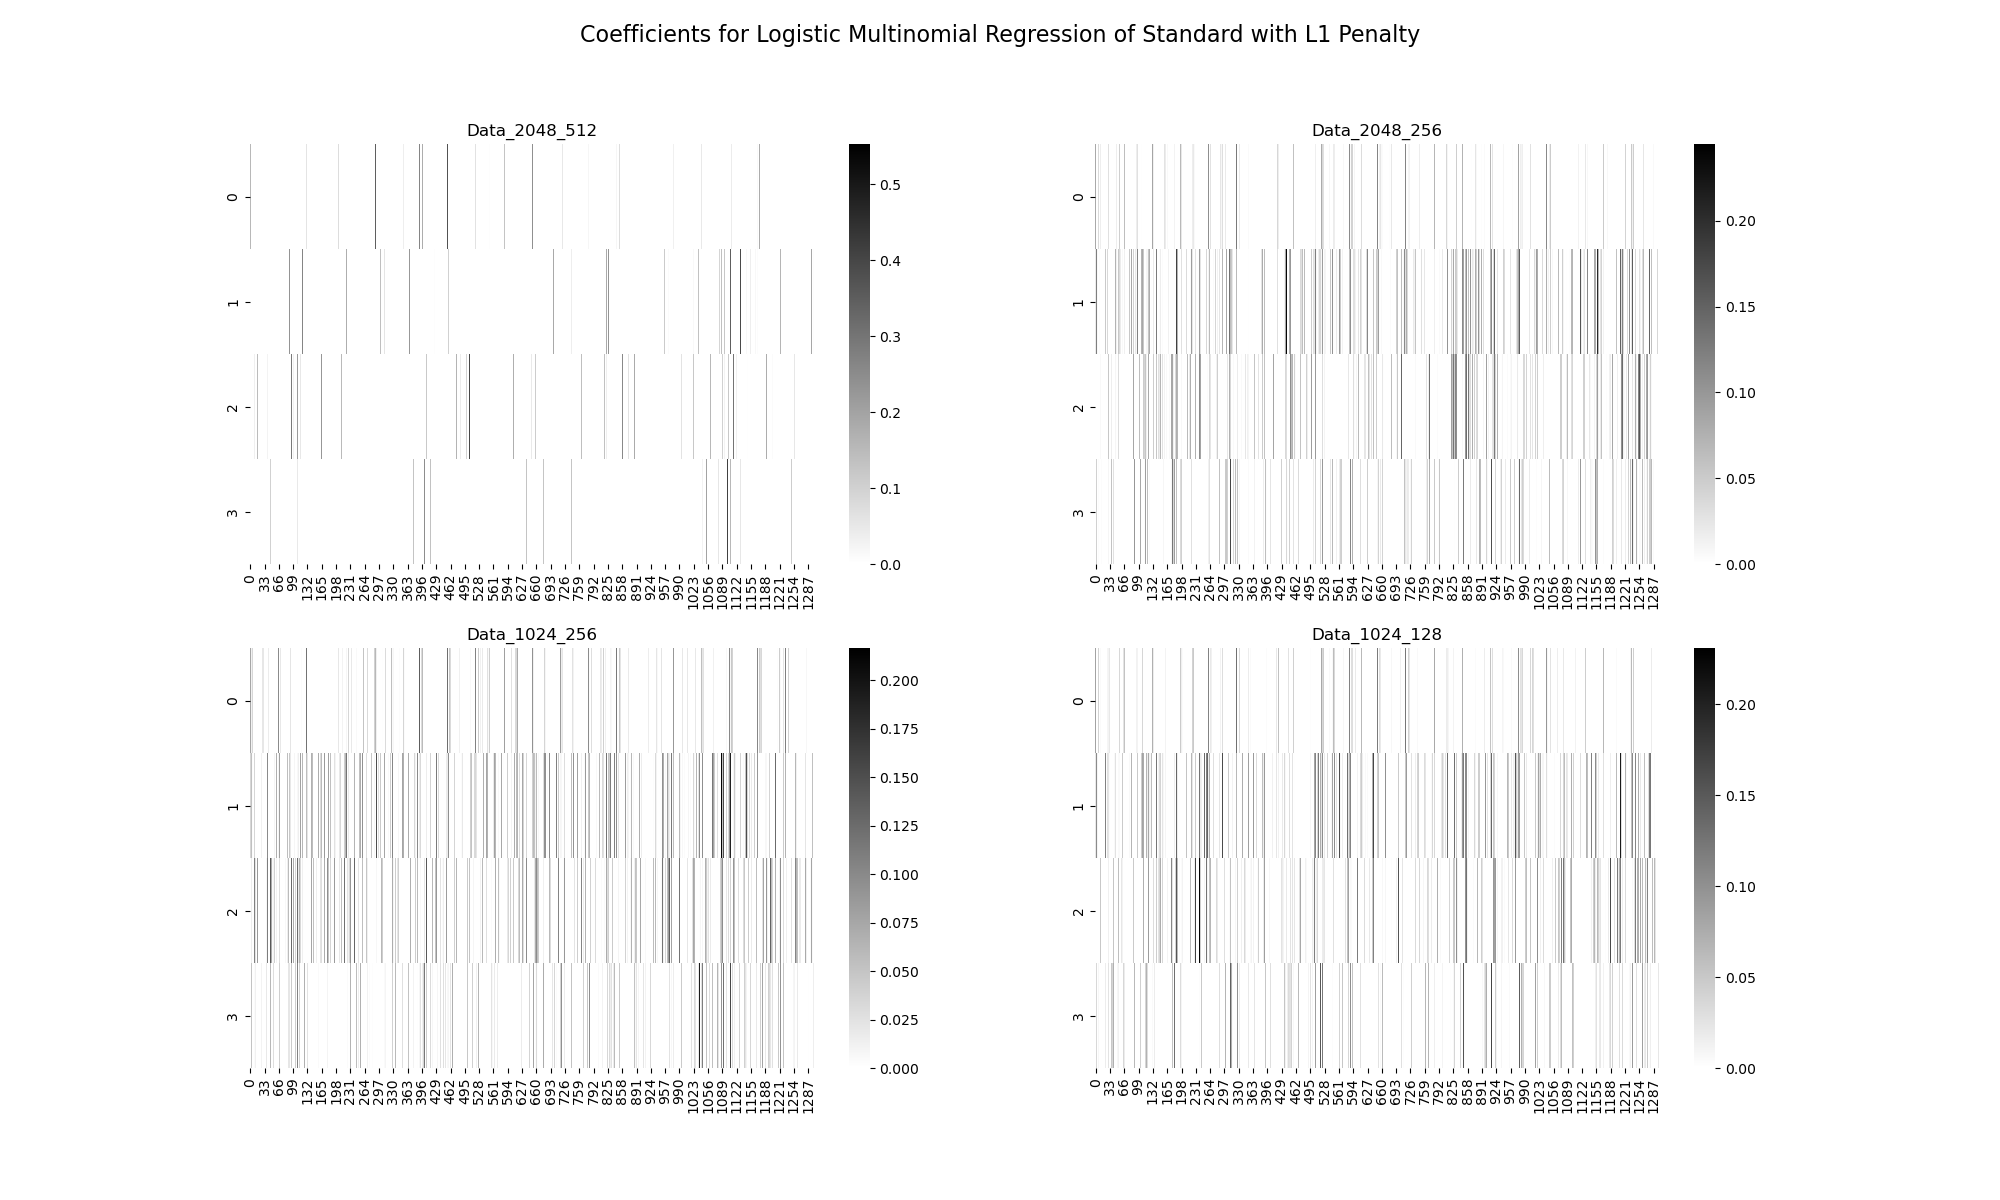
\includegraphics[width=0.9\linewidth]{../Statistical_Sciences_template/figure/Coefficients for Logistic Multinomial Regression of Standard with L1 Penalty.png}
	\caption{Coefficients for Multinomial Logistic Regression of Standard Datasets with L1 Penalty}
	\label{fig:MLRstdcoef}
\end{figure}
\noindent According to the numbers of the non-zero regression coefficients, we can further find that in the model of the dataset with frame length 2048 and hop length 512, the variables corresponding to non-zero coefficients show obvious differences: the most representative features of MFCCs' mean occupies a dominant position, with a total of 67 corresponding variables obtaining non-zero coefficients; followed by features related to the range, with 37 variables retained by the model, 42 variables corresponding to skewness, and 38 variables corresponding to kurtosis; in contrast, the variance feature describing the degree of dispersion performed the worst, with only 22 related variables selected by the model. In contrast, the model with the best results on the dataset with frame length 1024 and hop length 128, in which mean of MFCCs has a total of 335 related variables obtaining non-zero coefficients. The importance ranking of other statistics' types is consistent with the dataset with frame length 2048 and hop length 512, but the number scale has been significantly expanded: 274 variables of the range are retained, 286 of the skewness, and 288 of the kurtosis. The relative importance of the variance feature is still the lowest, with a total of 180 non-zero coefficients.\\
\\
Through comparative analysis of these models, we can draw the following important conclusion: first, the mean of MFCC shows the strongest discriminative ability among all statistics' types. This phenomenon may be due to the essential characteristics of the audio signal - the mean can effectively reflect the overall energy distribution of the signal, and this physical quantity often has a stable correlation with the audio category. Secondly, the performance of the variance feature is relatively weak. This may be because after standardization, the variance provides limited supplementary information, as larger variance means more information contained in data, hence the discriminative ability of variance is significantly weakened. Finally, although the statistics describing the distribution shape (skewness and kurtosis) and the value range are not as important as the mean, they still contain a considerable degree of discriminative information. These features can capture subtle differences in signal distribution and provide valuable supplementary information for the model.\\
\\
Figure \ref{fig:CMMLRstd} shows the confusion matrix performance of the best multinomial logistic regression model on the test set, where the category labels 0, 1, 2, and 3 correspond to classical, disco, hiphop, and metal respectively. Several important classification patterns can be observed from the confusion matrix: first, in the classical music category, the model shows perfect classification performance, and all test samples are correctly identified, which verifies the results in Section \ref{subsec:performance}. Second, the model only makes a few misclassifications between disco and hiphop, and between hiphop and mental, with only 3 observations misclassified in each case. However, the model has systematic biases in certain specific categories: for disco, the model shows a clear tendency to misclassify it as mental, with a total of 5 disco samples misclassified as mental. It is worth noting that this misclassification is asymmetric - there is no misclassification at all in the opposite direction (i.e. misclassifying mental as disco). This specific misclassification pattern directly affects the performance of the model's evaluation indicators: on the one hand, the recall of the disco is relatively lower because some of real disco samples are not correctly identified; on the other hand, the precision of the mental is also negatively affected because samples predicted as mental are mixed with samples that should belong to disco. This finding is completely consistent with the model performance indicators reported in Table \ref{table:best}.
\begin{figure}[H]
	\centering
	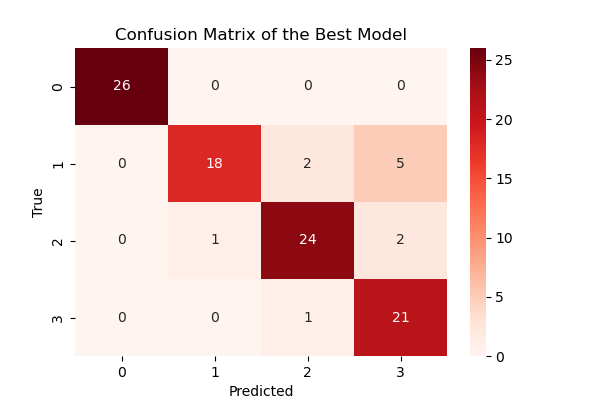
\includegraphics[width=0.9\linewidth]{../Statistical_Sciences_template/figure/Confusion matrix of the Best Model.png}
	\caption{Confusion matrix of the Best Model}
	\label{fig:CMMLRstd}
\end{figure}
\noindent For comparison, Figure \ref{fig:MLRcoef} shows a heat map of all coefficients in the multinomial logistic regression model based on unstandardized datasets. Through intuitive comparison, it can be found that the density of non-zero coefficients in Figure \ref{fig:MLRcoef} is significantly higher than that in Figure \ref{fig:MLRstdcoef}, which indicates that under unstandardized data conditions, the model tends to retain more variables. The results of the specific analysis of the dataset with frame length 1024 and hop length 128 show that variables related to the mean dominate the model, with a total of 1028 variables retained; since the data is not standardized, the importance of variance and range is also fully reflected in the model, of which 1037 non-zero coefficient variables corresponding to variance and 1031 corresponding to range. This shows that the number of variables corresponding to the three types of statistics, mean, variance and range, retained in the model is basically the same, the difference in the number of retained variables is less than 1\%, and their importance to the model is also relatively close. It is worth noting that the importance of skewness is significantly reduced, with only 68 related variables retained; while the number of variables corresponding to the kurtosis statistic is between the above two, with a total of 610 retained. This distribution pattern indicates that under unstandardized data conditions, the second-order moment statistics has a much greater impact on the model than higher-order statistics (i.e. skewness and kurtosis), which may be related to the original scale difference of the data.\\
\\
\begin{figure}[H]
	\centering
	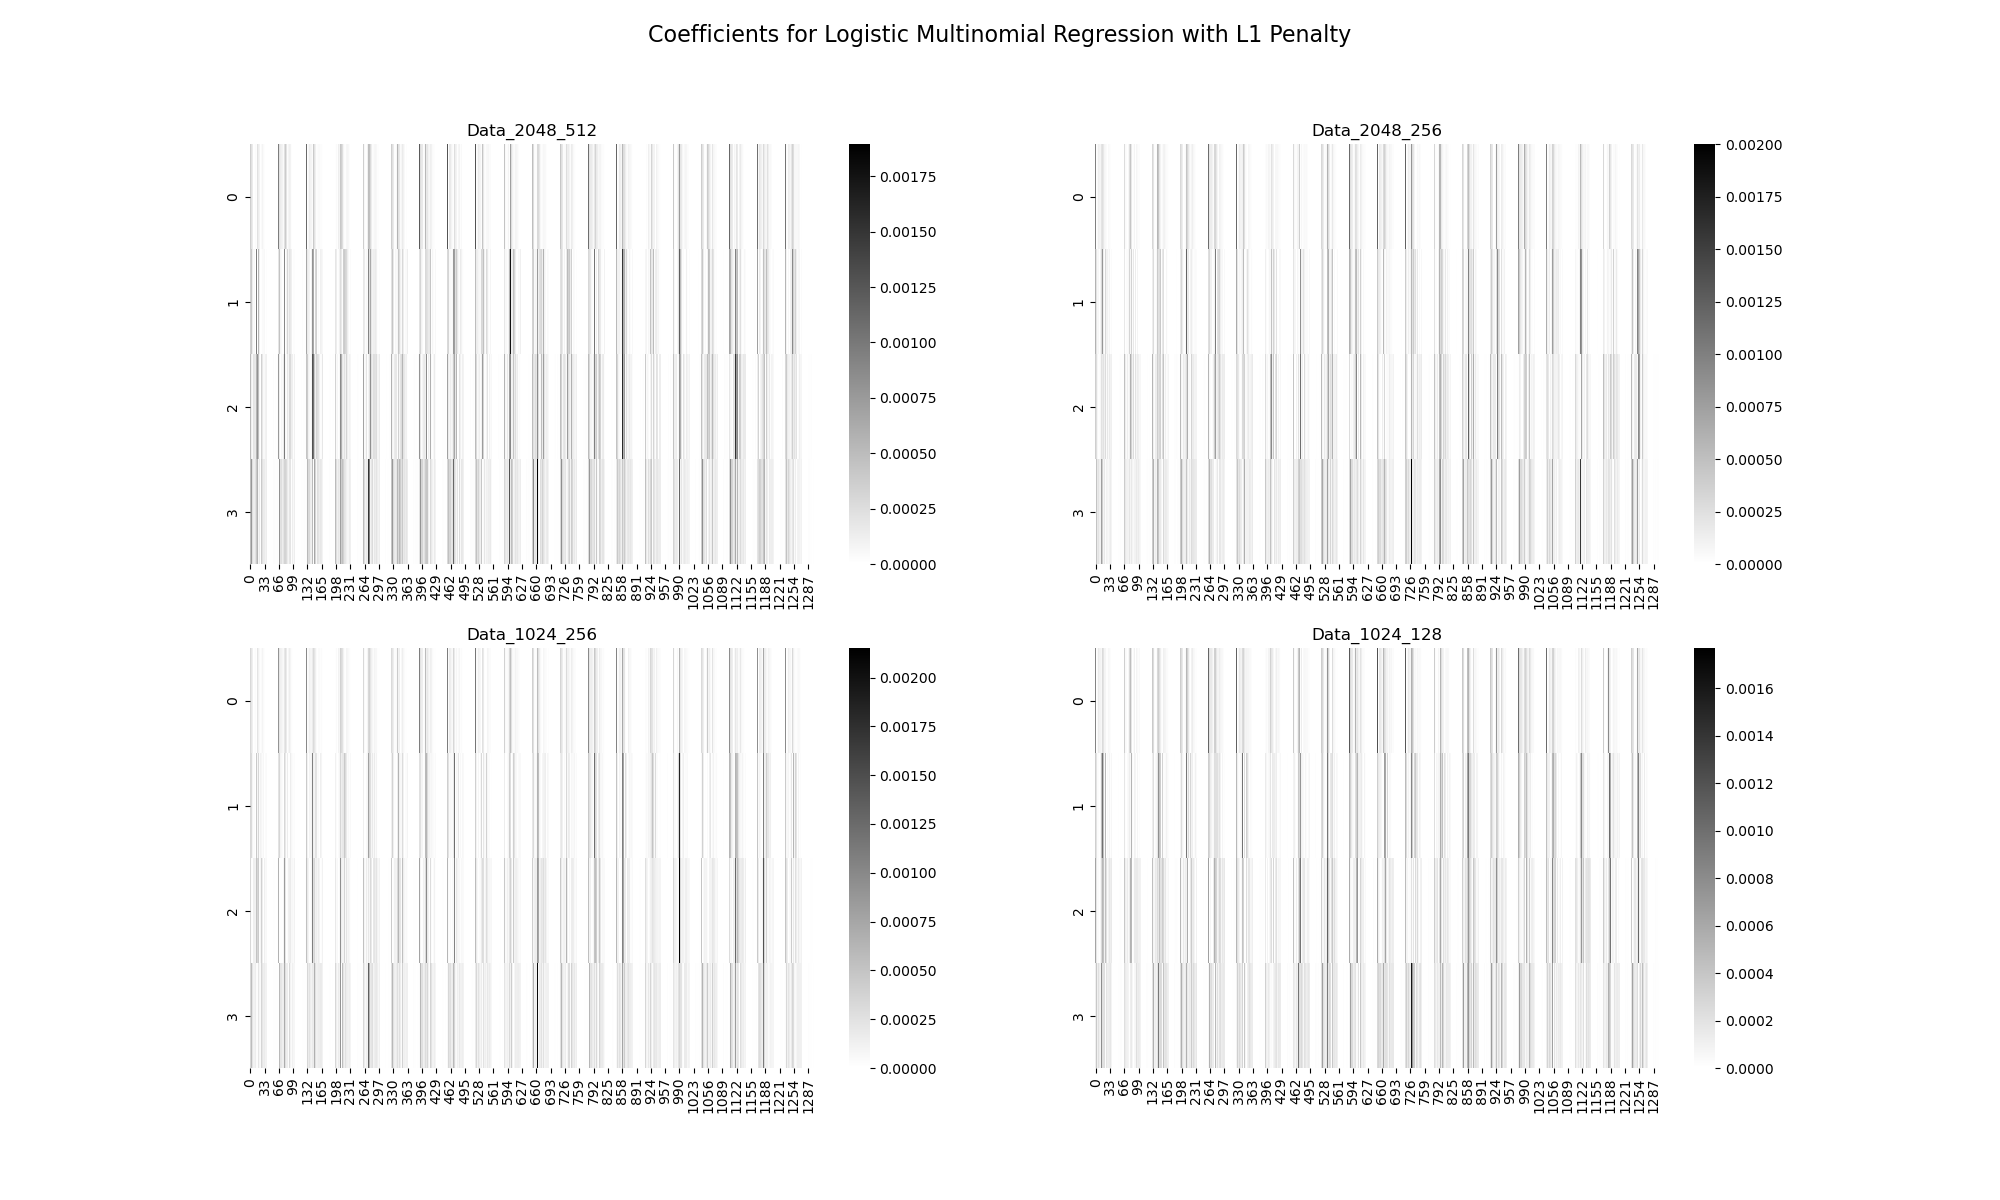
\includegraphics[width=0.9\linewidth]{../Statistical_Sciences_template/figure/Coefficients for Logistic Multinomial Regression with L1 Penalty.png}
	\caption{Coefficients for Logistic Regression of Unstandard Datasets with L1 Penalty}
	\label{fig:MLRcoef}
\end{figure}
\noindent From the performance comparison in Table \ref{table:L1penalty}, it can be seen that the models based on the unstandardized datasets performed significantly worse than the models based on the standardized datasets. Although more non-zero variables are retained in the unstandardized models, its prediction effect is worse, which may be mainly due to the fact that too many variables corresponding to variance are retained in the model. These variables are likely to be associated with noise, thus affecting the model performance. From the perspective of signal processing, STFT is used when calculating MFCCs, while STFT is based on the short-time stationarity assumption, that is, the second-order moment of the signal in the short-time window is required to remain constant. However, in actual situations, under the condition of unstandardized data, a large number of variables of MFCCs corresponding to variance are retained in the model, which not only squeezes out the importance of other statistical variables, but also these variables themselves may not contain enough information, but may introduce noise interference, ultimately leading to a decrease in model performance. In addition, due to the inconsistent scale of unstandardized data, some variables may be given higher weights simply because of their larger numerical range, rather than having stronger discrimination ability.\\
\\
In contrast, standardization achieves the unification of data scales, allowing the model to more effectively retain discriminative variables. This processing method eliminates the impact of dimensional differences between different features, allowing the model to more accurately capture the inherent laws of the data, thereby significantly improving the model's predictive performance. Standardized data allows various statistics to be compared at the same scale, avoiding unreasonable weights for certain features due to their large dimensions, and ensuring the objectivity and effectiveness of model learning. In addition, the standardization process may also suppress the interference of noise variables, allowing truly discriminative high-order statistics (i.e. skewness and kurtosis) to be more reasonably weighted in the model.\\
\\
Figure \ref{fig:SVMcoef} shows the heatmap of coefficients when SVM constructs a classification hyperplane in the feature space. Compared with the aforementioned regression model, these hyperplane coefficients show more sparse characteristics, but it is worth noting that the absolute values of non-zero coefficients are generally larger, and some coefficients even reach 0.3. This phenomenon is contrast to the regression model on the standardized data set, where the absolute values of regression coefficients on other datasets except the dataset with frame length 5048 and hop length 512 generally do not exceed 0.2. Further analysis shows that in the SVM model, the variables corresponding to the skewness and kurtosis statistics show stronger discrimination and importance. Taking the specific analysis of dataset with frame length 1024 and hop length 128 as an example, the number of non-zero coefficients related to skewness reaches 137, the number of non-zero coefficients related to kurtosis is 113, and the number of non-zero coefficients corresponding to mean, variance and range is significantly reduced, only 56, 46 and 53 respectively. This distribution pattern is essentially different from the results of the regression model: in regression analysis, variables corresponding to mean always dominate, but in the SVM classification task, high-order statistics (skewness and kurtosis) show stronger discrimination.\\
\\
\begin{figure}[H]
	\centering
	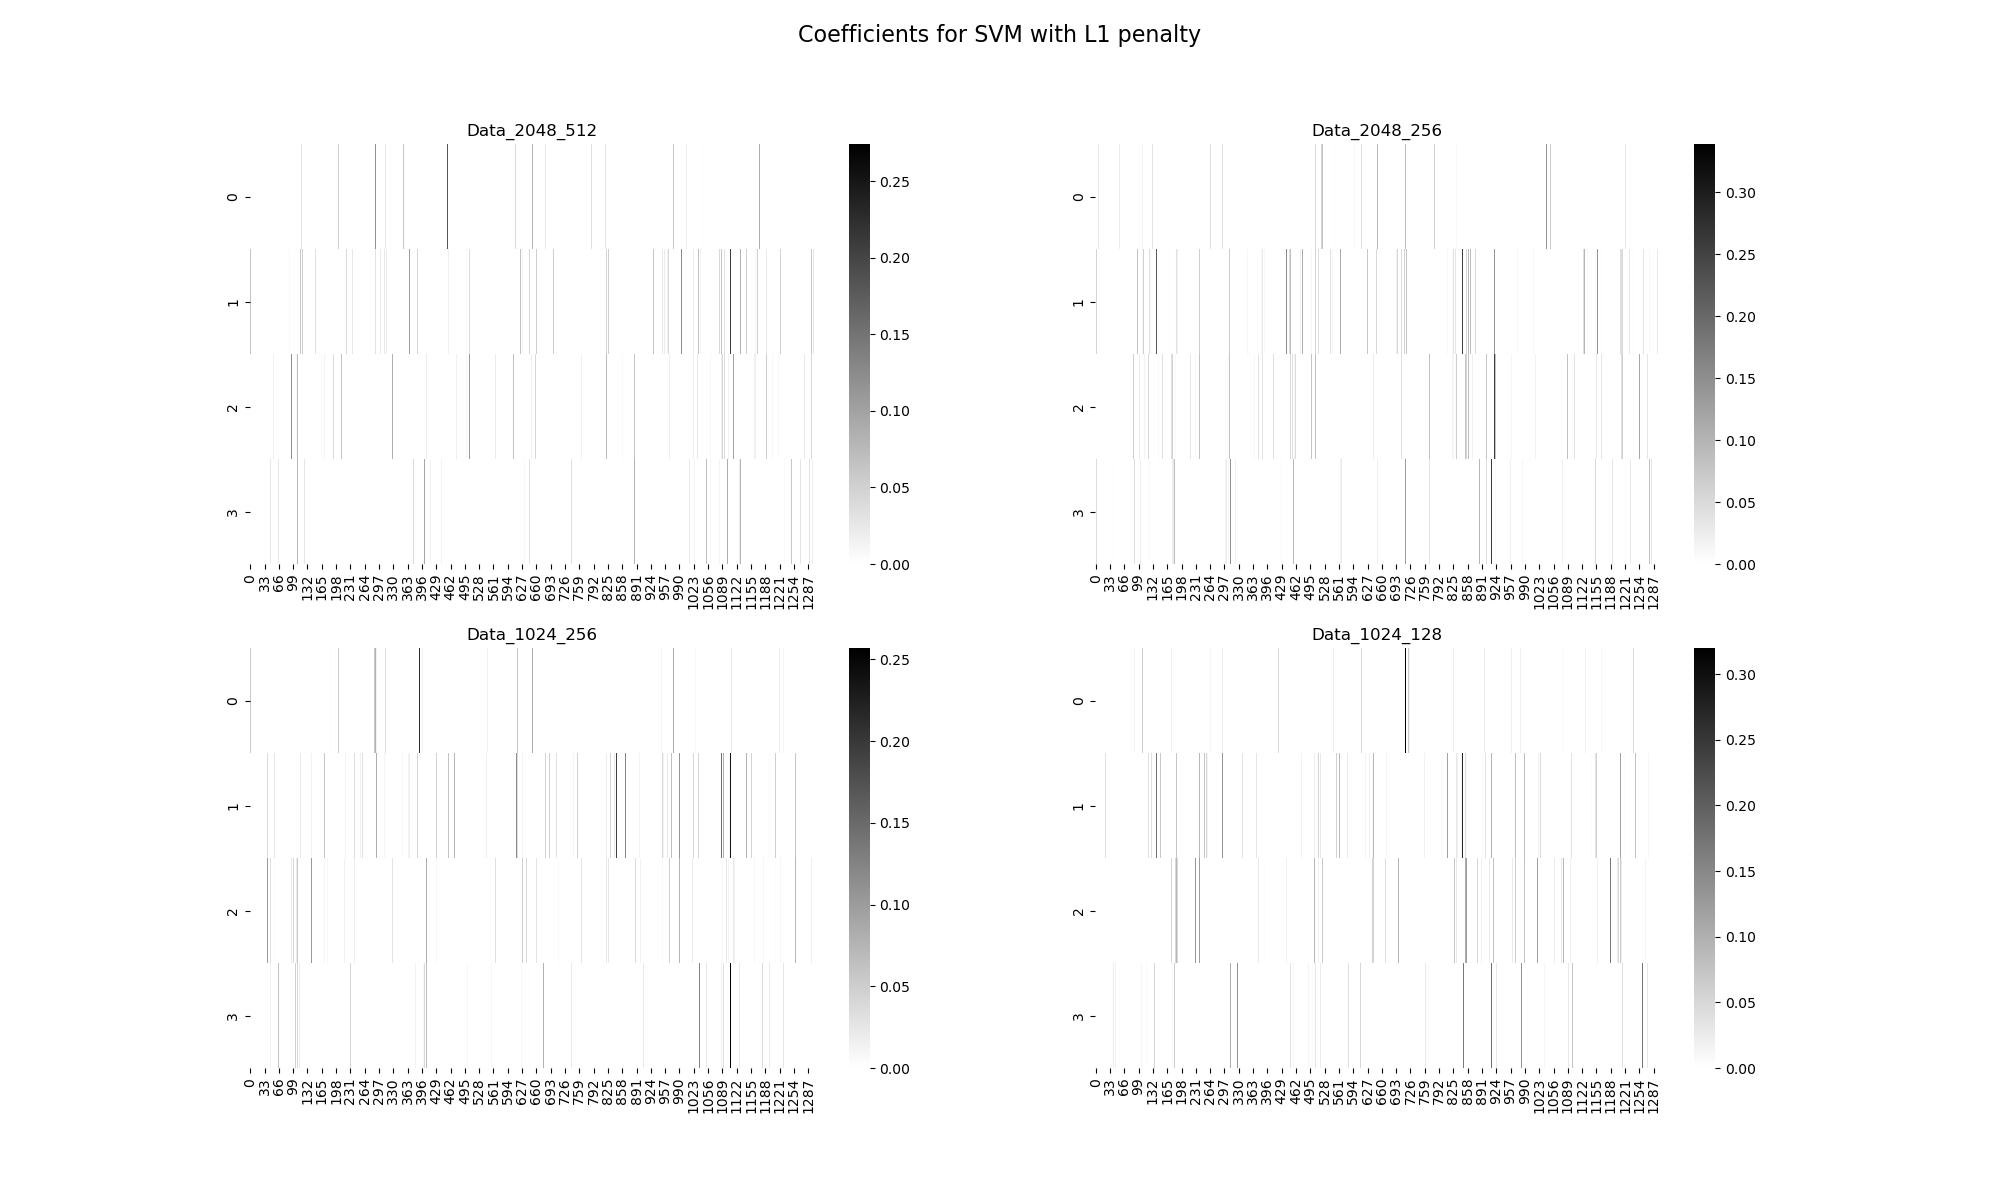
\includegraphics[width=0.9\linewidth]{../Statistical_Sciences_template/figure/Coefficients for SVM with L1 penalty.png}
	\caption{Coefficients for SVM with L1 penalty}
	\label{fig:SVMcoef}
\end{figure}
\noindent The best shapelet tree-based model constructed on the dataset with frame length 2048 and hop length 256 forms a decision tree structure with a depth of 3 as shown in Figure \ref{fig:shapelettree}. It can be clearly observed from the confusion matrix shown in Figure \ref{fig:CMshapelet} that the model has the best prediction performance for the classical, with only 3 observation samples being misclassified. In contrast, although the model has shown a certain degree of discrimination ability for the hiphop and mental, its prediction accuracy is lower than that of the classical category. It is particularly noteworthy that the model performs extremely poorly in the recognition of the disco, and is almost unable to effectively distinguish this category from other music types. This phenomenon can be explained by an in-depth analysis of the correspondence between the shapelet features shown in Figure \ref{fig:shapelets} and the time series of each category.\\
\\
\begin{center}
	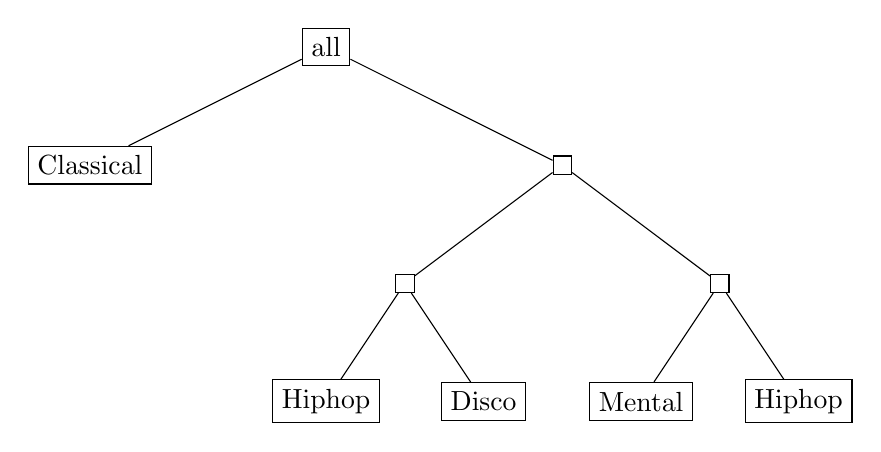
\begin{tikzpicture}[
        level 1/.style={sibling distance=6cm, level distance=1.5cm},
        level 2/.style={sibling distance=4cm, level distance=1.5cm},
        level 3/.style={sibling distance=2cm, level distance=1.5cm},
		every node/.style={draw, rectangle}
		]
		\node (Root) {all}
		child {node {Classical}
		}
		child {node {}
			child {node {}
				 child {node {Hiphop}}
				 child {node {Disco}}
			}
			child {node {} 
				child {node {Mental}} 
				child {node {Hiphop}}
			}
		};
	\end{tikzpicture}
	\label{fig:shapelettree}
\end{center}
\noindent The shapelet used by the parent node corresponds to the red curve in Figure \ref{fig:shapelets} that shows a fishhook shape. This feature has a large time span and significant amplitude changes. By comparing the time series features of each category, it can be found that classical music shows extremely significant amplitude fluctuations in the time period corresponding to this shapelet, especially in the low-frequency area (the part with lower values). This unique fluctuation pattern makes the distance measurement value between the classical music sequence and the fishhook shapelet significantly smaller than that of other categories, thus forming an effective basis for discrimination.\\
\\
\begin{figure}[H]
	\centering
	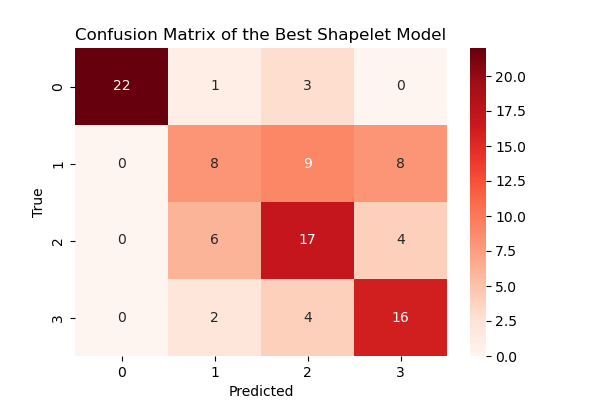
\includegraphics[width=0.9\linewidth]{../Statistical_Sciences_template/figure/Confusion matrix of the Best Shapelet Model.png}
	\caption{Confusion matrix of the Best Shapelet Model}
	\label{fig:CMshapelet}
\end{figure}
\noindent Further analysis of the discriminant features of the third layer of the decision tree shows that the shapelet used by the right child node (corresponding to the red curve starting from -57 and with a length of 9 time units in Figure \ref{fig:shapelets}) has a certain effect in distinguishing hiphop and mental categories. This shapelet is closer to the time series morphology of hiphop music, but has a more obvious morphological difference with the mental category. However, the shapelet used by another third-layer child node (corresponding to the red curve starting from -25 and with a length of 9 time units in Figure \ref{fig:shapelets}) shows poor representativeness. This feature is morphologically between the hiphop and disco categories and cannot form an effective discriminant boundary, which directly leads to the model's serious lack of recognition ability for the disco category. From the perspective of time series morphology, the distribution of disco music in this feature space has a large overlap with other categories, and lacks a unique and discriminative fluctuation pattern, which is the fundamental reason for the model's disastrous results in this category.
\begin{figure}[H]
	\centering
	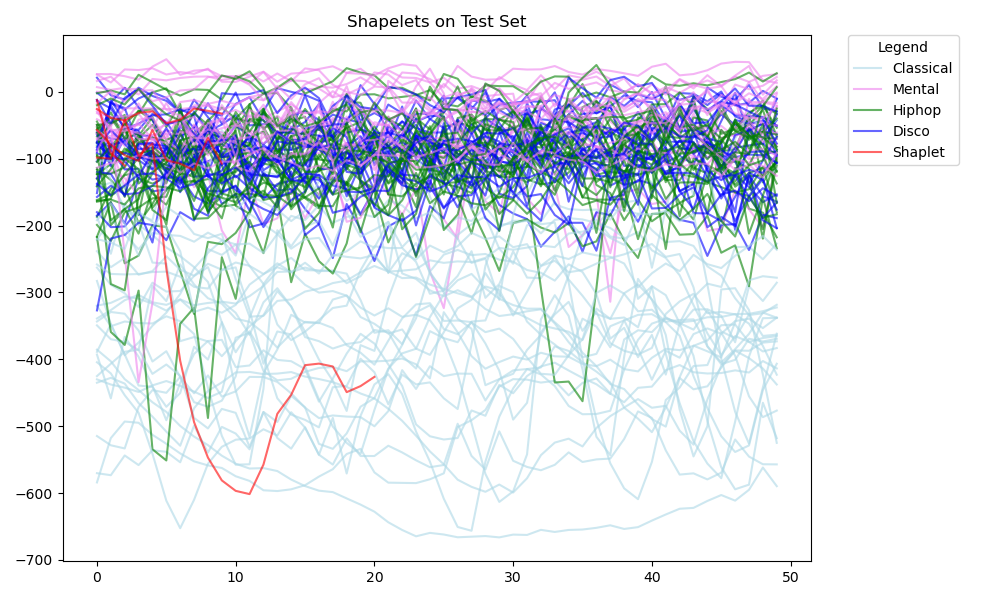
\includegraphics[width=0.9\linewidth]{../Statistical_Sciences_template/figure/Shapelets on Test Set.png}
	\caption{Shapelets and the Samples from Test Set}
	\label{fig:shapelets}
\end{figure}